% Options for packages loaded elsewhere
\PassOptionsToPackage{unicode}{hyperref}
\PassOptionsToPackage{hyphens}{url}
\PassOptionsToPackage{dvipsnames,svgnames*,x11names*}{xcolor}
%
\documentclass[
  11pt,
  openany]{book}
\usepackage{lmodern}
\usepackage{amsmath}
\usepackage{ifxetex,ifluatex}
\ifnum 0\ifxetex 1\fi\ifluatex 1\fi=0 % if pdftex
  \usepackage[T1]{fontenc}
  \usepackage[utf8]{inputenc}
  \usepackage{textcomp} % provide euro and other symbols
  \usepackage{amssymb}
\else % if luatex or xetex
  \usepackage{unicode-math}
  \defaultfontfeatures{Scale=MatchLowercase}
  \defaultfontfeatures[\rmfamily]{Ligatures=TeX,Scale=1}
  \setmainfont[]{Constantia}
  \setmonofont[Scale=0.8]{Source Code Pro}
\fi
% Use upquote if available, for straight quotes in verbatim environments
\IfFileExists{upquote.sty}{\usepackage{upquote}}{}
\IfFileExists{microtype.sty}{% use microtype if available
  \usepackage[]{microtype}
  \UseMicrotypeSet[protrusion]{basicmath} % disable protrusion for tt fonts
}{}
\makeatletter
\@ifundefined{KOMAClassName}{% if non-KOMA class
  \IfFileExists{parskip.sty}{%
    \usepackage{parskip}
  }{% else
    \setlength{\parindent}{0pt}
    \setlength{\parskip}{6pt plus 2pt minus 1pt}}
}{% if KOMA class
  \KOMAoptions{parskip=half}}
\makeatother
\usepackage{xcolor}
\IfFileExists{xurl.sty}{\usepackage{xurl}}{} % add URL line breaks if available
\IfFileExists{bookmark.sty}{\usepackage{bookmark}}{\usepackage{hyperref}}
\hypersetup{
  pdftitle={Stress Reactivity Disturbances of the Neurocardiac Axis},
  colorlinks=true,
  linkcolor=Maroon,
  filecolor=Maroon,
  citecolor=Blue,
  urlcolor=Blue,
  pdfcreator={LaTeX via pandoc}}
\urlstyle{same} % disable monospaced font for URLs
\usepackage[top=1in,bottom=1in,left=1.5in,right=1.5in]{geometry}
\usepackage{longtable,booktabs}
\usepackage{calc} % for calculating minipage widths
% Correct order of tables after \paragraph or \subparagraph
\usepackage{etoolbox}
\makeatletter
\patchcmd\longtable{\par}{\if@noskipsec\mbox{}\fi\par}{}{}
\makeatother
% Allow footnotes in longtable head/foot
\IfFileExists{footnotehyper.sty}{\usepackage{footnotehyper}}{\usepackage{footnote}}
\makesavenoteenv{longtable}
\usepackage{graphicx}
\makeatletter
\def\maxwidth{\ifdim\Gin@nat@width>\linewidth\linewidth\else\Gin@nat@width\fi}
\def\maxheight{\ifdim\Gin@nat@height>\textheight\textheight\else\Gin@nat@height\fi}
\makeatother
% Scale images if necessary, so that they will not overflow the page
% margins by default, and it is still possible to overwrite the defaults
% using explicit options in \includegraphics[width, height, ...]{}
\setkeys{Gin}{width=\maxwidth,height=\maxheight,keepaspectratio}
% Set default figure placement to htbp
\makeatletter
\def\fps@figure{htbp}
\makeatother
\setlength{\emergencystretch}{3em} % prevent overfull lines
\providecommand{\tightlist}{%
  \setlength{\itemsep}{0pt}\setlength{\parskip}{0pt}}
\setcounter{secnumdepth}{5}
% Remove "Chapter X" pattern
\usepackage{titlesec}
\titleformat{\chapter}
  {\normalfont\LARGE\bfseries}{\thechapter}{1em}{}
\titlespacing*{\chapter}{0pt}{3.5ex plus 1ex minus .2ex}{2.3ex plus .2ex}

% Short landscape command for both windows/mac
\usepackage{pdflscape}
\newcommand{\bland}{\begin{landscape}}
\newcommand{\eland}{\end{landscape}}

% Short footnote command for both windows/mac
\newcommand{\bfoot}{\begin{footnotesize}}
\newcommand{\efoot}{\end{footnotesize}}

% Handle spacing
\usepackage[none]{hyphenat}
%\raggedbottom
\usepackage{setspace}
\doublespacing

% Commenting out sections
\usepackage{comment}
\AtBeginDocument{\frontmatter}
\usepackage{float}
\usepackage{longtable}
\usepackage{booktabs}
\usepackage{array}
\usepackage{multirow}
\usepackage{wrapfig}
\usepackage{float}
\usepackage{colortbl}
\usepackage{tabu}
\usepackage{threeparttable}
\usepackage{threeparttablex}
\usepackage[normalem]{ulem}
\usepackage{makecell}
\usepackage{xcolor}
\usepackage{graphicx}
\usepackage{amsmath}
\usepackage{booktabs}
\usepackage{caption}
\usepackage{longtable}
\ifluatex
  \usepackage{selnolig}  % disable illegal ligatures
\fi
\newlength{\cslhangindent}
\setlength{\cslhangindent}{1.5em}
\newlength{\csllabelwidth}
\setlength{\csllabelwidth}{3em}
\newenvironment{CSLReferences}[2] % #1 hanging-ident, #2 entry spacing
 {% don't indent paragraphs
  \setlength{\parindent}{0pt}
  % turn on hanging indent if param 1 is 1
  \ifodd #1 \everypar{\setlength{\hangindent}{\cslhangindent}}\ignorespaces\fi
  % set entry spacing
  \ifnum #2 > 0
  \setlength{\parskip}{#2\baselineskip}
  \fi
 }%
 {}
\usepackage{calc}
\newcommand{\CSLBlock}[1]{#1\hfill\break}
\newcommand{\CSLLeftMargin}[1]{\parbox[t]{\csllabelwidth}{#1}}
\newcommand{\CSLRightInline}[1]{\parbox[t]{\linewidth - \csllabelwidth}{#1}\break}
\newcommand{\CSLIndent}[1]{\hspace{\cslhangindent}#1}

\title{Stress Reactivity\\
Disturbances of the Neurocardiac Axis}
\usepackage{etoolbox}
\makeatletter
\providecommand{\subtitle}[1]{% add subtitle to \maketitle
  \apptocmd{\@title}{\par {\large #1 \par}}{}{}
}
\makeatother
\subtitle{Anish Sanjay Shah}
\author{A thesis submitted for the degree of\\
\emph{Master of Science in Clinical Research}\\
Laney Graduate School\\
Emory University}
\date{2021-03-16}

\begin{document}
\maketitle

\begin{singlespace}
\tableofcontents
\end{singlespace}

\hypertarget{acknowledgements}{%
\chapter{Acknowledgements}\label{acknowledgements}}

Foremost, I would like to thank my mentors and mentoring team. Dr.~Shah has been a tremendous supporter of my academic growth, and has challenged me to continue to explore and learn, and create an area of academic excellence for myself. Dr.~Alonso and Dr.~Thames have all supported my efforts through direct mentorship and academic guidance. Dr.~Quyyumi and Dr.~Vaccarino have created a research environment that has laid the groundwork for these projects.

Second, I would like to thank the support staff that has allowed this research to unfold, from the EPICORE group with Nancy Murrah and Lucy Shallenberger, to the MSCR program with Cheryl Sroka and the outstanding MSCR instructors.

Finally, I would like to thank my family for their patience and support.

\hypertarget{abbreviations}{%
\chapter{Abbreviations}\label{abbreviations}}

There are several key abbreviations that will be used throughout. They have been outlined here for reference.

\bfoot

\captionsetup[table]{labelformat=empty,skip=1pt}
\begin{longtable}{ll}
\toprule
Term & Abbreviation \\ 
\midrule
ANS & Autonomic Nervous System \\ 
Biobank & Emory Cardiovascular Biobank \\ 
CAD & Coronary Artery Disease \\ 
CFR & Coronary Flow Reserve \\ 
HRV & Heart Rate Variability \\ 
MACE & Major Adverse Cardiovascular Events \\ 
MI & Myocardial Infarction \\ 
MIMS & Myocardial Infarction and Mental Stress \\ 
MIPS & Mental Stress Ischemia Prognosis Study \\ 
MPI & Myocardial Perfusion Imaging \\ 
MSIMI & Mental Stress-Induced Myocardial Ischemia \\ 
PSIMI & Physical Stress-Induced Myocardial Ischemia \\ 
PTSD & Post-Traumatic Stress Disorder \\ 
Twins & Emory Twins Study \\ 
\bottomrule
\end{longtable}

\efoot

\mainmatter

\hypertarget{part-introduction}{%
\part*{INTRODUCTION}\label{part-introduction}}
\addcontentsline{toc}{part}{INTRODUCTION}

\hypertarget{the-problem}{%
\chapter{The Problem}\label{the-problem}}

\begin{quote}
``Why did he die on Tuesday and not on Monday?''

--- Douglas Zipes
\end{quote}

The underlying premise in this question posed by Dr.~Zipes is that the cardiac substrate can be \emph{triggered} into an catastrophic maelstrom (\protect\hyperlink{ref-Zipes2006}{1}).
That trigger is oftentimes psychological in nature, and in the right setting, such as a scarred myocardium, can lead to electrical instability and ventricular arrhythmias (\protect\hyperlink{ref-Lown1979}{2}).
The reaction of the body to such stresses is thus a critical step in the pathogenesis of major adverse cardiovascular events.

Patients with psychiatric disease have an increased of cardiovascular disease and overall mortality (\protect\hyperlink{ref-Carney2002}{3},\protect\hyperlink{ref-Boscarino2008}{4}).
Depression, for example, is the leading cause of disabilty in the world (\protect\hyperlink{ref-Friedrich2017b}{5}), and coronary artery disease (CAD) is the leading cause of death (\protect\hyperlink{ref-McAloon2016b}{6}).
The prevalence of depression is 20\% in patients with CAD, and in those with comorbid depression and CAD, there is a 3-fold increase in cardiovascular mortality (\protect\hyperlink{ref-Jha2019}{7},\protect\hyperlink{ref-Meijer2011}{8}).
Thus, understanding how the body reacts to stress can have implications in the the pathogenesis of the increased cardiovascular risk seen in psychological disease.

The purpose of this dissertation is to assess how physiological and psychological stress can be measured, and whether or not these measures of stress are clinically pertinent.
Measuring stress and stress reactivity requires a method to quantify disturbances of the neurocardiac axis, and assessing changes from both a neuropsychological and cardiac perspective (\protect\hyperlink{ref-Davis1993}{9}).
Leveraging different types of stress along the neurocardiac axis is important, such as the effect of myocardial ischemia, acute mental stress, chronic psychological stress, and systemic diurnal changes.

\hypertarget{the-approach}{%
\chapter{The Approach}\label{the-approach}}

The suspected mechanism of behind stress reactivity is through dysfunction of the autonomic nervous system (ANS), particularly as there is an increased mortality with known ANS dysfunction (\protect\hyperlink{ref-LaRovere1998}{10},\protect\hyperlink{ref-Stein2000}{11}).
Both psychological stress and myocardial ischemia are known to have a relationship with ANS dysfunction (\protect\hyperlink{ref-Carney2005}{12}), and the interaction between sympathetic and parasympathetic nervous activity is thus consequential.

To measure ANS dysfunction, a common surrogate is through electrocardiographic (ECG) changes based on sympathetic and vagal effects upon the sinoatrial node, or pacemaker, of the heart.
The corresponding heart rate variability (HRV), and its mathematical derivatives, can thus inform us of the dynamic changes to autonomic tone (\protect\hyperlink{ref-Sassi2015}{13}).
By measuring autonomic tone during different stress, we can quantify the stress reactivity of the phenomenon and model its impact on clinically relevant factors, such as depression, cardiovascular disease, and major adverse cardiovascular events.

\hypertarget{part-background}{%
\part*{BACKGROUND}\label{part-background}}
\addcontentsline{toc}{part}{BACKGROUND}

\hypertarget{clinical-importance}{%
\chapter{Clinical Importance}\label{clinical-importance}}

Psychological stress is increasingly recognized as an important potentially modifiable risk factor for cardiovascular disease (\protect\hyperlink{ref-Steptoe2012}{14}).
Psychiatric disease leads to an increase cardiovascular disease and overall mortality.
PTSD, for example, has twice the hazard ratio for not only progressive coronary artery disease, but also for overall mortality (\protect\hyperlink{ref-Boscarino2008}{4}).
Depression and loneliness have a distinct increase in all-cause mortality (\protect\hyperlink{ref-Steptoe2013a}{15}), and almost twice twice the risk of coronary artery disease (\protect\hyperlink{ref-Ford1998}{16}).
Specifically, depression is the leading cause of disability worldwide, estimated to be prevalent in over 300 million people, which accounts for roughly 4\% of the global population (\protect\hyperlink{ref-Friedrich2017b}{5}).
In the United States, the estimated economic burden of depression is \$210 billion dollars as of 2010, doubling in cost from 2000 (\protect\hyperlink{ref-Greenberg2015b}{17}), suggesting a worsening, growing burden.
CAD on the other hand remains the leading cause of death (\protect\hyperlink{ref-McAloon2016b}{6}).
This corresponds with approximately \$204 billion dollars of estimated direct and indirect costs, with both continuing to climb (\protect\hyperlink{ref-Benjamin2018c}{18}).

In individuals with CAD, the prevalence of depression is estimated to be 20\%, and in those with comorbid depression and CAD, there is over a 3-fold increase in cardiovascular mortality (\protect\hyperlink{ref-Jha2019}{7},\protect\hyperlink{ref-Meijer2011}{8}).
This increased risk of mortality in CAD with depression has remained unchanged over the past 35 years (\protect\hyperlink{ref-Carney2017}{19}), as only in recent years has depression been considered an additional prognostic marker of mortality in CAD (\protect\hyperlink{ref-Lichtman2014}{20}).

Although interventions such as cognitive behavioral therapy and antidepressants are well-proven in reducing symptoms of psychological distress, their impacts are only modest in patients with CAD, and they do not impact event-free survival (\protect\hyperlink{ref-Berkman2003}{21}).
Although the American College of Cardiology recommends depression should be routinely screened for in patients with cardiovascular disease, there is limited evidence that this leads to an improvement in overall mortality (\protect\hyperlink{ref-Kronish2019}{22}).
More research is needed to understand the therapeutic mechanism underlying psychological distress and CAD (\protect\hyperlink{ref-Carney2017}{19}), as there are no effective therapies for these high-risk individuals in comorbid patients.

The causal mechanism is suspected to be through ANS dysfunction, as this has been found to occur in both diseases of the brain and heart (\protect\hyperlink{ref-Davis1993}{9}).
Not only are somatic symptoms of psychological stress predictive of cardiovascular mortality, but they may be explained by changes seen in HRV (\protect\hyperlink{ref-Smolderen2017}{23},\protect\hyperlink{ref-Shah2021a}{24}).
Similarly, abnormalities in myocardial perfusion are related to and may be predated by abnormalities in HRV (\protect\hyperlink{ref-Shah2020}{26}).
Thus, investigating the role of autonomic dysfunction in neurocardiac disorders is both mechanistically plausible and may allow for the development of efficacious therapeutic interventions.

\hypertarget{relevant-literature}{%
\chapter{Relevant Literature}\label{relevant-literature}}

The heart itself harbors an intrinsic cardiac nervous system that responds to changes in autonomic tone, such as in myocardial ischemia and infarction, by changing chronotropic, inotropic, and dromotropic responses (\protect\hyperlink{ref-Armour1999}{27},\protect\hyperlink{ref-Zipes1990}{28}).
Autonomic dysfunction occurs at multiple levels, from central neurological processes to cardiovascular reflexes (\protect\hyperlink{ref-Abboud2011}{29}).
This includes vagal withdrawal seen in depression and heigtened sympathetic tone seen in PTSD or cardiovascular disease.
Depression, for example, has been linked to dysregulation of the ANS through changes in levels of catecholamines (\protect\hyperlink{ref-Veith1994b}{30}), increased cardiovascular reactivity to stress (\protect\hyperlink{ref-Hughes2008}{31}), and decreased baroreflex sensitivity (\protect\hyperlink{ref-Davydov2007}{32}).

ANS-related mechanisms are important as they may inform future therapies.
In the past, stellectomy was found to reduce angina pectoris and ventricular dysrhythmias (\protect\hyperlink{ref-Schwartz2017a}{33}).
Modern interventions have shown to improve symptom burden in both depression and CAD (\protect\hyperlink{ref-Penninx2017}{34}).
Vagal nerve stimulation has been shown to relieve cardiac arrhythmias, and has been effective against treatment-resistant depression (\protect\hyperlink{ref-Zhang2011a}{35}).
In PTSD, non-invasive vagal nerve stimulation has also been found to blunt the sympathetic response to stress (\protect\hyperlink{ref-Gurel2019a}{36}).

HRV has been shown to be an effective ECG-based biomarker for ANS dysfunction.
HRV is an accepted measure of autonomic activity, as it is an integration of sympathetic and parasympathetic efferent input at the level of the sinoatrial node (\protect\hyperlink{ref-Saul1990}{37}).
For example, the non-linear HRV marker of \emph{Dyx} has been shown to predict ventricular dysrhythmia and cardiovascular mortality after myocardial infarction, with a hazard ratio of 2.4 (95\% CI 1.5 --- 3.8) (\protect\hyperlink{ref-Juxf8rgensen2016}{38}).
In addition, individuals with chest pain and abnormal \emph{Dyx} had an odds ratio of 8 (95\% CI 3.1 --- 23.99) for abnormal exercise stress test (\protect\hyperlink{ref-Goldkorn2015b}{39}).
Not only does HRV correlate well with cardiovascular disease, but is strongly correlated with depression (\protect\hyperlink{ref-Stein2000}{11}).
This relationship between psychological stress, cardiovascular disease, and the autonomic nervous system is thus an appropriate candidate for further investigation, particularly in justifying the clinical utility in measuing autonomic dysfunction (\protect\hyperlink{ref-Carney2005}{12}).
In addition to chronic mental stress, acute mental stress has become a more common way of assessing physiological reactivity.
Mental stress has been shown to associate with chronic psychological stressors (\protect\hyperlink{ref-Petrowski2016}{40}), and can also lead to the development of myocardial ischemia (\protect\hyperlink{ref-Arri2016}{41}).
This phenomenon, known as mental stress-induced myocardial ischemia (MSIMI), is an important reaction to stress that has been shown to predict long-term clinical outcomes (\protect\hyperlink{ref-Vaccarino2018}{42}).
HRV has been shown that to associate with acute mental stress (\protect\hyperlink{ref-Castaldo2015}{43}), but the relationship between MSIMI has not yet been determined.

The circadian rhythm in autonomic dysfunction is also relevant. The response to the stress of changing from sleep to wake has been seen to associate with increased cardiovascular mortality.
There is an increased frequency of sudden cardiac death based on time of day, usually peaking between 6 AM and 10 AM (\protect\hyperlink{ref-Muller1999}{44},\protect\hyperlink{ref-Boudreau2011}{45}), with a secondary peak between 6 PM and 8 PM (\protect\hyperlink{ref-Mulcahy1988}{46}).
There is a circadian pattern to autonomic outflow, melatonin, cortisol, and circulating catecholamines which could increase vulnerability to ischemia and cardiac death during morning hours {[}(\protect\hyperlink{ref-Boudreau2011}{45}); Scheer2010{]}.
The relationship of circadian changes in HRV and myocardial perfusion has been shown to be related (\protect\hyperlink{ref-Shah2020}{26}), but how circadian changes may be important in psychological stress and overall mortality is not yet known.

\hypertarget{part-methods}{%
\part*{METHODS}\label{part-methods}}
\addcontentsline{toc}{part}{METHODS}

\hypertarget{aims}{%
\chapter{Specific Aims}\label{aims}}

The response to both physiological and psychological stress can be markers of overall cardiovascular adaptability. The following aims help to assess the clinical importance of stress reactivity as measured by disturbances to the neurocardiac axis.

\begin{enumerate}
\def\labelenumi{\arabic{enumi}.}
\tightlist
\item
  To assess the association between myocardial ischemia and coronary perfusion on cardiac autonomic activity.
\item
  To determine if cardiac autonomic activity modifies the relationship between acute and chronic psychological stress and myocardial ischemia.
\item
  To explore the association of cardiac autonomic activity with future major adverse cardiovascular events.
\end{enumerate}

To achieve these aims, we will leverage the several data sets, including the Emory Cardiovascular Biobank (\emph{Biobank}), the Myocardial Infarction and Mental Stress (\emph{MIMS}) and Mental Stress Ischemia Prognosis Study (\emph{MIPS}), and the Emory Twins Study (\emph{Twins}). Each of these data sets contribute variations of coronary artery physiology, acute and chronic mental stressors, and electrocardiographic data of varying recording lengths.

\hypertarget{study-design}{%
\chapter{Study Design}\label{study-design}}

\hypertarget{population-characteristics-and-study-overview}{%
\section{Population Characteristics and Study Overview}\label{population-characteristics-and-study-overview}}

\hypertarget{emory-cardiovascular-biobank}{%
\subsection{Emory Cardiovascular Biobank}\label{emory-cardiovascular-biobank}}

The \emph{Biobank} studies major cardiovascular events, and also evaluates additional biomarkers for inflammation, cardiac injury, and genetics, with the goal of predicting CVD outcomes (\protect\hyperlink{ref-Ko2017}{47}).
All patients aged 18 years and older undergoing cardiac catherization were included.
During the index cardiac catheterization, additional measures including lifestyle factors, psychological status, medical comorbidities, revascularization and previous procedures were ascertained via patient interview and chart review.
Additionally, ambulatory ECG was collected with the VivaLNK patch, which was placed on the morning of cardiac catheterization and removed after catheterization for up to 24 h of data recording.
Patients were excluded if they have congenital heart disease, severe valvular heart disease, severe anemia, a recent blood transfusion, myocarditis, history of active inflammatory disease, cancer or are unable or not willing to provide consent (approximately 5\%).
Those that are found to have atrial fibrillation or have \textgreater20\% ectopic beat burden or noise, as well as those that are pacer dependent were excluded.
Those with known CAD were also excluded.

\hypertarget{emory-twins-study}{%
\subsection{Emory Twins Study}\label{emory-twins-study}}

The \emph{Twins} is a cross-sectional study was designed to evaluate the relationship of abnormal stress myocardial perfusion with autonomic function, measured hourly over the course of 24 h, in individuals without known ischemic heart disease.
Subjects were drawn from the Emory Twin Study, which recruited middle-aged male twin pairs from the Vietnam Era Twin Registry (\protect\hyperlink{ref-Shah2013}{48}--\protect\hyperlink{ref-Goldberg2002}{50}).
Pairs of twins were examined at the Emory University General Clinical Research Center, and all data collection occurred during a 24-hour admission under controlled conditions.
The twins in each pair maintained a nearly identical schedule, with all data collection beginning and ending at the same time.
The twins arrived at 11 AM, with ECG recording started at approximately 1 PM, questionnaires and exam performed between 2 and 4 PM, dinner at 5 PM, bedtime at 10 PM, wake-up time at 6:30 AM, and PET scans performed between 8 and 10 AM the following morning.
The twins were followed longitudinally for follow-up events, including review of national registries, which were adjudicated.
Subjects were excluded from analysis if they were unable to complete pharmacological stress testing.

\hypertarget{mental-stress-ischemia-mechanisms-and-prognosis-myocardial-infarction-and-mental-stress}{%
\subsection{Mental Stress Ischemia Mechanisms and Prognosis, Myocardial Infarction and Mental Stress}\label{mental-stress-ischemia-mechanisms-and-prognosis-myocardial-infarction-and-mental-stress}}

The study design has been described prior, and is the same between the two cohorts (\protect\hyperlink{ref-Hammadah2017a}{51}).
The \emph{MIMS} cohorts had recent myocardial ischemia within the 8 months prior to enrollment and were younger than 61 years of age at time of screening.
The \emph{MIPS} cohort included patients with stable CAD diagnosed via coronary angiogram, documented MI, or positive nuclear stress test.
All patients underwent mental stress test and physical stress test using either treadmill or regadenosine, and were randomly assigned to complete one and then the other in two separate visits within a week.
During the initial visit, medical history and psychological assessments were performed as well.
During the mental stress testing, all patients had ECG recordings made of variable duration.
Patients were followed longitudinally for 3-5 years for follow-up events, which were adjudicated.
Patients were excluded for having acute coronary syndrome or decompensated heart failure, severe psychiatric conditions other than depression, pregnancy, uncontrolled high blood pressure, or contraindications to pharmacological stress testing.

\hypertarget{measurements}{%
\section{Measurements}\label{measurements}}

\hypertarget{electrocardiography-measures}{%
\subsection{Electrocardiography Measures}\label{electrocardiography-measures}}

In all three cohorts, ECG data was collected and analyzed using similar techniques. As described, in the \emph{Biobank}, ECG was collected through a single, bipolar lead using the VivaLNK patch, with data being recorded for up to 24 h. In the \emph{Twins}, ambulatory ECG was collected through Holter monitor (GE Marquette SEER digital system; GE Medical Systems, Waukesha, Wisconsin) for 24 h. Holter monitor was also used in the \emph{MIMS/MIPS}, however the recording time was only for several hours.

Variations in heart rate can be assessed by a number of mathematical measures, usually divided into the time and frequency domains (\protect\hyperlink{ref-TaskForceoftheESCandNAS1996a}{52}).
HRV was calculated through the Physionet Cardiovascular Signal Toolbox (\protect\hyperlink{ref-Vest2018}{53}), which is an open-source MATLAB software for analyzing ECG signal.
Time domain measures we used include the RR interval duration (converted to heart rate in beats-per-minute), the standard deviation of normally conducted RR intervals (SDNN), the root mean square of successive differences in normally conducted RR intervals (RMSSD), and the proportion of normally conducted RR intervals that differ by more than 50 ms divided by the total number of normally conducted RR intervals (PNN50).
Frequency-domain measures computed through power spectral analysis categorize variability as very low frequency (VLF, 0.0033 to \textless0.04 Hz), low frequency (LF, 0.04 to \textless0.15 Hz) or high frequency (HF, 0.15 to 0.40 Hz) (\protect\hyperlink{ref-Akselrod1981}{54}).
These frequency categories reflect autonomically mediated heart rate responses to physiologic stimuli, including influences of the renin-angiotensin-aldosterone system, baroreceptor activity, and respiration (\protect\hyperlink{ref-Akselrod1981}{54}).
The sympathetic and parasympathetic nervous systems influence them to different degrees.
HF reflects primarily parasympathetic nervous system activity, while LF reflects both sympathetic and parasympathetic activity (\protect\hyperlink{ref-ReyesdelPaso2013}{55}).
Total power HRV is a nonspecific global measure.
RMSSD is an approximate correlate of HF, and SDNN is an approximate correlate of TP, supporting the physiological basis of these markers.{[}Electrophysiology1996b{]}
Acceleration capacity and deceleration capacity were also included where available, based on signal quality and recording length, as they also reflect clinically relevant sympathetic and vagal activity (\protect\hyperlink{ref-Bauer2006c}{56}).
These metrics are well-known as physiologic markers of acute and chronic stress, and measure slightly different aspects of autonomic nervous system function.
HRV was also analyzed hourly through the commercial HeartTrends algorithm (Lev-El Diagnostics Ltd, Israel), which generated the \emph{Dyx} measure.
\emph{Dyx} is derived from heart rate time series analysis and measures the variability and randomness of the heart rhythm.
\emph{Dyx} is generated through the multipole method analysis of Poincaré plot, in which beat-to-beat (RR) interval lengths are plotted as a function of prior RR intervals to form an ellipse, as seen in Figure \ref{FigurePoincare}.
\emph{Dyx} is calculated as the ratio of the kurtosis along the y-axis (long-term variability) and the x-axis (beat-to-beat random variation) of the ellipse, and higher values indicate more beat-to-beat randomness and/or decreased variability (\protect\hyperlink{ref-Olesen2005}{57},\protect\hyperlink{ref-Lewkowicz2002}{58}).

In addition to summary and hourly assessments of HRV, diurnal rhythms were examined using cosinor metrics within the \emph{Twins} (\protect\hyperlink{ref-Refinetti2007}{59}). Morphological assessment of ECG changes were also performed in the \emph{MIMS/MIPS} with T-wave area.

\hypertarget{psychological-measures}{%
\subsection{Psychological Measures}\label{psychological-measures}}

In all cohorts, chronic psychological variables were measured through patient interviews.
In the \emph{Biobank}, depressive symptoms were assessed via the 9-question Primary Care Evaluation of Mental Disorders Brief Patient Health Questionnaire (PHQ-9) (\protect\hyperlink{ref-Kroenke2001}{60}).
Moderate-severe depression is considered when the PHQ-9 score is 10 points or higher (out of 27), with this cutpoint having a sensitivity and specificity of 88\% for major depression.
Within the \emph{Twins} and \emph{MIMS/MIPS} cohorts, depressive symptomers were assessed with Beck's Depression Inventory, which includes 21 items with 4 statements scored 0-3, with higher scores indicating higher severity of depression (\protect\hyperlink{ref-Beck1988}{61}).
A cut-off of \(\geq\) 14 points was used to identify patients with moderate-to-severe depressive symptom burden.
The diagnosis of post-traumatic stress disorder (PTSD) was defined using the Structured Clinical Interview for Diagnostic and Statistical Manual of Mental Disorders, 4th Edition (DSM-IV) (\protect\hyperlink{ref-First2004}{62}).

In the \emph{MIMS/MIPS} cohort, there was a separate protocol for acute mental stress challenge.
Patients were initially allowed to rest for 30 minutes in a calm, quiet, dimly lit, and temperature-regulated room.
After the resting period, mental stress was induced by a standardized public speaking task, as previously described (\protect\hyperlink{ref-DavidGoldberg1996}{63}).
The patients were asked to imagine a real-life stressful situation, such as a close relative having been mistreated in a nursing home, and then asked to make up a realistic story around this scenario.
They were given two minutes to prepare the statement, and three minutes to present it in front of a video camera and an audience.
The patients were told that the speech would be evaluated for content, quality, and duration.

\hypertarget{cardiac-measures}{%
\subsection{Cardiac Measures}\label{cardiac-measures}}

All cohorts underwent imaging of the heart through different modalities, which all assess complementary aspects of myocardial blood flow.

The \emph{Biobank} used direct coronary angiography through cardiac catheterization.
Obstructive CAD was defined as \(\ge\) 70\% stenosis or hemodynamic significance by fractional flow reserve.
Coronary angiography was used to determine the Gensini score, which is a visual estimation of luminal narrowing in multiple segments based on a modified form of the American Heart Association classification of the coronary tree by trained cardiologists (\protect\hyperlink{ref-Gensini1983}{64}).
Coronary angiography was also evaluated using the Coronary Artery Surgery Study (CASS), which evaluates the number of major epicardial vessels that have a certain percent stenosis, e.g.~the CASS-50 score determines the number of vessels with \(\ge\) 50\% stenosis (\protect\hyperlink{ref-Ringqvist1983}{65}).
Importantly, direct coronary angiography is limited to visualization of the large, epicardial conduit vessels.

The \emph{Twins} study used MPI using underwent MPI using nitrogen-13-ammonia positron emission tomography (PET) with adenosine as the pharmacologic stressor.
Adenosine doses were calculated to induce maximal coronary vasodilation (\protect\hyperlink{ref-Vaccarino2011}{66}).
Areas of diminished uptake indicate reduced capacity to maximally vasodilate, thereby causing relative coronary hypoperfusion.
Images were visually interpreted by experienced cardiologists and radiologists with training in nuclear cardiology.
Quantitative analysis was performed with the Emory Cardiac Toolbox to generate: a) coronary flow reserve (CFR) for absolute myocardial blood flow during stress and rest, and b) the stress total severity score (STSS), which measures the sum of the number of standard deviations below the expected value for each pixel compared to a database of normal controls (\protect\hyperlink{ref-Hutchins1990}{67}).
CFR was defined as the ratio of mean stress to rest myocardial blood flow (mL/min/g), and low CFR was defined as a ratio \(<\) 1.5 (\protect\hyperlink{ref-Gould2018a}{68}).
Abnormal MPI findings were defined as \(>\) 5\% MPI deficit.
For generalizability, semi-quantitative assessments were used.

In the \emph{MIMS/MIPS}, MPI was also used but with single-photon emission computered tomography (SPECT), using sestamibi radio-labelled with Technetium-99.
SPECT was performed at rest, after mental stress, and after physical stress (either exercise or pharmacological).
Myocardial perfusion abnormalities were quantified using the Emory Cardiac Toolbox software, similar to the \emph{Twins}, and semi-quantitative assessments were determined.

\hypertarget{sample-size-and-power-considerations}{%
\section{Sample Size and Power Considerations}\label{sample-size-and-power-considerations}}

The subjects for the \emph{Biobank} were enrolled from September 2019 to February 2020, however further enrollment was limited due to the COVID-19 pandemic.
It was expected that approximately 200 patients would be needed for adequate power, but due to limitations, the analyses were conducted on available data.
The enrollment for \emph{MIMS/MIPS} and \emph{Twins} was completed prior to the initiation of this analysis, and provided a robust population to expand upon and answer the specific aims.

\hypertarget{analysis}{%
\chapter{Analysis}\label{analysis}}

Statistical analysis was performed using R 4.0.0 (R Core Team 2020, Vienna, Austria).
The analytical approach was guided by the specific aims (Section \ref{aims}).

\hypertarget{clinical-characteristics}{%
\section{Clinical Characteristics}\label{clinical-characteristics}}

In the \emph{Biobank}, HRV was summarized over the recording length and at 15-30 minute intervals at the time of coronary angiography.
In the \emph{Twins}, HRV was computed hourly, including \emph{Dyx}.
The 24-hour data was used to generate cosinor statistics as well using published software (\protect\hyperlink{ref-Shah2020d}{69}).
In the \emph{MIMS/MIPS}, HRV was computed for each phase of the mental stress challenge.
Power spectral density measures of HF, LF, and VLF HRV were log-transformed for normal distribution.
Each of the clinical cohorts was described by clinical covariates, including frequency of comorbid diseases and summary statistics of continuous measures.

\hypertarget{myocardial-ischemia}{%
\section{Myocardial Ischemia}\label{myocardial-ischemia}}

The purpose of \textbf{Aim I} was to identify the relationship of autonomic dysfunction with CAD, as measured by both coronary angiography and MPI.
Within the \emph{Biobank}, summary HRV metrics were compared between those with obstructive CAD versus nonobstructive CAD using the Wilcoxon rank sum test.
HRV was then assess in a similar manner between those receiving revascularization and those that did not.
HRV was segmented by timing of coronary angiography.
HRV was compared at the start of catheterization (or initial intervention in those that were revascularized) to the 30 minutes before the procedure, by intervention status.

To evaluate the relationship with myocardial perfusion, HRV was also assessed within the \emph{MIMS/MIPS} cohort, which had both mental and physical stress MPI as outcomes.
Logistic regressions were used with HRV during stress and rest as the exposures, not adjusted for clinical covariates.
The area under the receiver-operator characteristic curves were generated.

\[
\begin{aligned}
  \operatorname{global\_cfr}_{i}  &\sim N \left(\mu, \sigma^2 \right) \\
    \mu &=\alpha_{j[i],k[i]} + \beta_{1}(\operatorname{lf}) + \beta_{2}(\operatorname{age}) + \beta_{3}(\operatorname{bmi})\ + \\
&\quad \beta_{4}(\operatorname{race}_{\operatorname{African\ American}}) + \beta_{5}(\operatorname{race}_{\operatorname{Asian}}) + \beta_{6}(\operatorname{smoking}_{\operatorname{1}}) + \beta_{7}(\operatorname{prevchd}_{\operatorname{1}})\ + \\
&\quad \beta_{9}(\operatorname{hptn}_{\operatorname{1}}) + \beta_{0}(\operatorname{dm}_{\operatorname{1}}) \\
    \alpha_{j}  &\sim N \left(\mu_{\alpha_{j}}, \sigma^2_{\alpha_{j}} \right)
    \text{, for vetrid j = 1,} \dots \text{,J} \\
    \alpha_{k}  &\sim N \left(\gamma_{0}^{\alpha} + \gamma_{1}^{\alpha}(\operatorname{chf}_{\operatorname{1}}), \sigma^2_{\alpha_{k}} \right)
    \text{, for pair k = 1,} \dots \text{,K}
\end{aligned}
\]

Within the \emph{Twins}, similar analyses were performed with MPI and hourly HRV. Early morning, approximately 7 AM, HRV was used based on previous work suggesting the strong temporal relationship of HRV with clinical outcomes (\protect\hyperlink{ref-Shah2020}{26}).
Generalized linear mixed-effects models with Laplace approximations were used to account for clustering within twin pairs and within repeat study visits (\protect\hyperlink{ref-Carlin2005a}{70}).
Coronary flow reserve was treated as the outcome variable in linear models, and abnormal MPI was treated as the outcome variable in logistic models.
With the mixed-effects model, with random effects or conditioning for both twin pair status and repeat study visits.
The models were sequentially adjusted for demographic variables (age, BMI, and race), and then for cardiovascular risk factors (smoking, hypertension, cardiovascular disease).
HRV was summarized as cosinor metrics of MESOR (midline estimating statistic of rhythm), amplitude, and acrophase.
These metrics were treated as exposures, with CFR and MPI as outcomes, in mixed effects models as above.

\hypertarget{psychological-stress}{%
\section{Psychological Stress}\label{psychological-stress}}

The purpose of \textbf{Aim II} was to establish the relationship between psychological stress and autonomic dysfunction.
Acute psychological stress was defined as the mental stress challenge in the \emph{MIMS/MIPS} cohorts. Chronic psychological stress was defined as diagnoses of depression and PTSD, and/or symptom burden.

In the \emph{Biobank}, the distribution of HRV was compared between those with depression, as measured by PHQ-9, using Wilcoxon rank sum test.
In the \emph{Twins}, using the above described generalized linear mixed-effects models, regression analysis was performed with early morning HRV as the exposure and either PTSD or depression as the outcome.
Sequential adjustment was performed for demographic factors and cardiovascular risk factors.
Cosinor metrics were also used as additional exposure variables in additional mixed-models.

The \emph{MIMS/MIPS} cohort offered the opportunity to assess both acute and chronic psychological stress.
The distribution of HRV was visually compared between phases of the mental stress challenge for all subjects.
HRV was then analyzed within subjects by comparing the rest phase to the both the stress and recovery phase using paired T-test.
The distribution of HRV was then compared by phase in those with MSIMI and those without MSIMI using the Wilcoxon rank sum test.
Logistic regression models were used with PTSD and depression as outcomes and HRV by stress phase as exposures, without adjustment, and concordance statistics were generated.
Logistic regression models were then built with MSIMI as the outcome and stress HRV as the exposure, along with concordance statistics.
These models were sequentially adjusted for demographic factors (age, BMI, sex, race), cardiovascular risk factors (smoking, hypertension, diabetes, hyperlipidemia), known cardiovascular disease (coronary/peripheral artery disease), and then with chronic psychological stress (depression, PTSD).

\hypertarget{clinical-outcomes}{%
\section{Clinical Outcomes}\label{clinical-outcomes}}

The purpose of \textbf{Aim III} was to evaluate the role of autonomic dysfunction in clinical outcomes, and understand the effect of autonomic dysfunction on the relationship between outcomes and both psychological stress and myocardial ischemia. Clinical outcomes were available in the \emph{Twins} and \emph{MIMS/MIPS} cohorts. Proportional hazard assumptions were assessed visually in both cohorts.

The clinical outcomes of interest were overall mortality and death by cardiovascular disease in the \emph{Twins}.
Early morning HRV was treated as the exposure, with the survival time before censoring event as the outcome in Cox proportional hazard models.
The models were sequentially adjusted for myocardial ischemia, demographic factors (age, BMI, race), cardiovascular factors (known cardiovascular disease, hypertension, diabetes, smoking), and psychological factors (depression, PTSD).
In a similar fashion, cosinor metrics for HRV were used as exposure variables in models that were sequentially adjusted as above.

In the \emph{MIMS/MIPS}, the clinical outcomes of interest were overall mortality, cardiovascular mortality, and recurrent cardiovascular events including myocardial infarction or revascularization.
Cox proportional hazard models were used for both overall and cardiovascular mortality.
Recurrent event analysis used proportional hazard models with strata for events and individuals using marginal models, Prentice-Williams-Peterson models (both total and gap time), and Anderson-Gill models (\protect\hyperlink{ref-Amorim2015a}{71}).
These models were sequentially adjusted for demographic factors (age, BMI, sex, race), cardiovascular risk factors (smoking, hypertension, diabetes, hyperlipidemia), known cardiovascular disease (coronary/peripheral artery disease), and then with chronic psychological stress (depression, PTSD).

\hypertarget{part-results}{%
\part*{RESULTS}\label{part-results}}
\addcontentsline{toc}{part}{RESULTS}

\hypertarget{clinical-characteristics-1}{%
\chapter{Clinical Characteristics}\label{clinical-characteristics-1}}

The study populations in the three cohorts are uniquely suited for these analyses. They are complementary in their description of cardiovascular disease, autonomic function, and psychological factors, and are described here.

The \emph{Biobank} cohort, as described in Table \ref{TableOneBiobank}, had 56 participants, with a mean (95\% CI) age in years of 62 (52, 70).
9 (17\%) were female, and 14 (26\%) were Black.
There were 34 (71\%) that had obstructive CAD on coronary angiography, and 10 (21\%) had depression.

The \emph{MIMS/MIPS} cohort had 958 participants.
The mean age was 59 (52, 68), 323 (34\%) were female, and 385 (41\%) were Black.
700 (84\%) had obstructive CAD.
273 (30\%) had a diagnosis of depression, and 87 (9.5\%) had a diagnosis of PTSD.
In this population, 238 (25\%) had MSIMI.
Additional breakdown by study group is described in \ref{TableOneMims}.

The \emph{Twins} cohort, as described in both Table \ref{TableOneTwins} and \ref{TableTwinsHRV}, had 1012 participants over 4 follow-up visits, with 610 unique participants.
The mean age was 55.0 (52.0, 57.0) during the initial enrollment period, and was 68.4 (66.8, 69.5) during the final enrollment period.
All participants were male, and 95.75\% were White.
The average rate over the enrollment periods of abnormal MPI was 12.13\%.
The average rate of PTSD was 16.52\% and the average rate of depression was 13.38\%.

\hypertarget{myocardial-ischemia-1}{%
\chapter{Myocardial Ischemia}\label{myocardial-ischemia-1}}

The relationship of autonomic dysfunction to CAD as measured by coronary angiography was assessed in the \emph{Biobank} cohort.
When comparing summary HRV metrics between those with obstructive CAD versus nonobstructive CAD, there were no significant differences between HRV distributions (\ref{TableBiobankCAD}).
When comparing those that had revascularization of the CAD and those that did not (\ref{TableBiobankRevasc}), there was a difference seen in RR interval.
Those that underwent revascularization had a mean (95\% CI) RR interval of 868 (775, 932), while those that did not had a mean RR interval of 648 (608, 872).
There was a trend towards an increased \emph{Dyx} in those that underwent revascularization (2.03 (1.52, 2.71)) than those that did not (1.36 (1.17, 1.78)).
No other HRV metrics were associated with revascularization.
To effect of the timing of revascularization on the subsequent changes in HRV acutely were assessed, as described in Table \ref{TableBiobankTiming}.
No differences were seen between HRV before or after cardiac catheterization.

The relationship of autonomic dysfunction to qualitative MPI was assessed using both mental stress and physical stress in the \emph{MIMS/MIPS} cohorts.
ECG and HRV metrics did not have an association with abnormal MPI with combined mental and physical stress nor with physical stress.
Both lf HRV and LF HRV most prominently had an association with MSIMI, with stress HRV HRV having an odds ratio (OR) = 0.48 (95\% CI 0.31, 0.76) and LF HRV having an OR = 0.45 (95\% CI 0.27, 0.74).
The other associations are described in Table \ref{TableMimsStress}.

This relationship between myocardial perfusion and autonomic dysfunction was further explored using quantitative MPI in the \emph{Twins} cohort.
Morning HRV at approximately 7 AM was predominately associated with coronary flow reserve, as described in Table \ref{TableTwinsMPI}.
A change in 1 unit of LF HRV was associated with an 1.16 (95\% CI 1.04, 1.28) in adjusted models.
\emph{Dyx} had an OR = 0.7 (95\% CI 0.51, 0.98) for abnormal MPI.

Within the \emph{Twins}, diurnal HRV metrics were measured using cosinor analysis.
The relationship of the MESOR, amplitude, and acrophase with abnormal MPI and coronary flow reserve were evaluated (Table \ref{TableTwinsCircMPI}).
The MESOR in particular showed a consistent relationship with coronary flow reserve, with a 0.88 (0.58, 1.32) increase in every 1 unit increase in LF HRV, and a 0.89 (0.61, 1.31) increase for every 1 unit increase in \emph{Dyx}.

\hypertarget{psychological-stress-1}{%
\chapter{Psychological Stress}\label{psychological-stress-1}}

Chronic psychological stressors were analyzed using all three cohorts.
In the \emph{Biobank} cohort, there were no significant differences seen in HRV by depressive symptoms as measured on the PHQ-9.

In the \emph{Twins}, early morning HRV was measured against both PTSD and depression.
There was a significant relationship between HRV and both depression and PTSD as seen in Table \ref{TableTwinsPsych}.
In adjusted logistic models for PTSD, every 1 unit increase in HF HRV had an OR = 0.57 (95\% CI 0.4, 0.82), and LF HRV had an OR = 0.65 (95\% CI 0.45, 0.94).
In adjusted models logistic models for depression, every 1 unit of increase in VLF HRV had an OR = 0.04 (95\% CI 0, 0.92).
\emph{Dyx} and VLF HRV were not strongly associated with PTSD.

WHen using the diurnal HRV metrics, measured by cosinor analysis, significant relationships were seen with both depression and PTSD in the MESOR and amplitude (Table \ref{TableTwinsCircPsych}).
For example, every 1 unit increase in the MESOR of LF HRV had an OR = 0.46 (95\% 0.31, 0.69) and every 1 unit increase in the amplitude had an OR = 0.31 (95\% 0.13, 0.72) for PTSD.
Every 1 unit increase in the MESOR of LF HRV had an OR = 0.26 (95\% 0.15, 0.45) and every 1 unit increase in the amplitude had an OR = 0.31 (95\% 0.14, 0.68) for depression.

Acute mental stress was also assessed primarily using the \emph{MIMS/MIPS} cohorts.
The distribution of HRV metrics based on the phase of acute mental stress challenge was evaluated, as seen in Figure \ref{FigureMimsViolin}.
There were small differences between stress and rest HRV, as seen in Table \ref{TableMimsPaired}.
The difference in distribution of HRV was compared between those that had MSIMI and those that did not, as described in \ref{TableMimsHRV}.
There was a decrease in HRV in those with MSIMI compared to those without, except with heart rate.

The association between HRV during acute mental stress and chronic mental stress was also assessed (Table \ref{TableMimsPsych}).
Every 10 beat/minute increase in resting heart rate had an OR = 1.33 (95\% CI 1.11, 1.58) for PTSD and an OR = 1.15 (95\% CI 1.01, 1.3) for depression.
Every 1 unit increase in LF HRV during recovery had an OR = 0.51 (95\% CI 0.26, 1.07) for depression.
No other HRV metrics were strongly associated.

To assess the relationship of acute mental stress with myocardial perfusion abnormalities, the relationship between HRV and MSIMI was assessed. As seen in Table \ref{TableMimsMSIMI}, there was a robust association between LF and HF HRV during rest and stress with MSIMI. In fully adjusted models, including adjustment for both cardiovascular and psychological risk factors, every 1 unit increase in stress HF HRV had an OR = 0.47 (95\% CI 0.29, 0.77) and stress LF HRV had an OR = 0.47 (95\% CI 0.3, 0.91) for MSIMI.

\hypertarget{clinical-outcomes-1}{%
\chapter{Clinical Outcomes}\label{clinical-outcomes-1}}

Clinical outcome data was available in both the \emph{Twins} and the \emph{MIMS/MIPS} cohorts.
With the \emph{Twins}, early morning HRV showed a robust association with overall mortality and with cardiovascular disease, as seen in Table \ref{TableTwinsOutcomes}.
In fully adjusted models for overall mortality, \emph{Dyx} and VLF HRV had the strongest association.
With every 1 unit of increase in \emph{Dyx}, there was a hazard ratio (HR) = 0.41 (95\% CI 0.27, 0.64), and with every 1 unit increase in VLF HRV, there was a HR = 0.49 (95\% CI 0.27, 0.88).
When evaluating the relationship of circadian changes in HRV and clinical outcomes, \emph{Dyx} was a significant predictor of both overall and cardiovascular mortality.
The MESOR of \emph{Dyx} had a HR = 0.34 (95\% CI 0.21, 0.56) and the amplitude of \emph{Dyx} had a HR = 0.42 (95\% CI 0.22, 0.79).
Further relationships are outlined in \ref{TableTwinsCircOutcomes}.

Using the \emph{MIMS/MIPS} cohorts, stress HRV was compared with clinical outcomes.
There was a robust relationship between stress HRV and overall mortality, cardiovascular mortality, and recurrent cardiovascular events as described in Table \ref{TableMimsOutcomes}.
In fully adjusted models for cardiovascular mortality, including adjustment for MSIMI, 1 unit increase in stress LF HRV had a HR = 0.25 (95\% CI 0.11, 0.56) and HF HRV had a HR = 0.25 (95\% CI 0.11, 0.56).

\hypertarget{part-discussion}{%
\part*{DISCUSSION}\label{part-discussion}}
\addcontentsline{toc}{part}{DISCUSSION}

\hypertarget{major-findings}{%
\chapter{Major Findings}\label{major-findings}}

\begin{itemize}
\item
  Aim 1: HRV and MPI/CAD on cath
\item
  Aim 2: HRV and acute/chronic mental stress
\item
  Aim 3: HRV and MACE
\item
  HRV not associated with obstructive CAD or percent stenosis
\item
  MPI however is strongly related, particularly with mental stress (MSIMI)
\item
  CFR and HRV more strongly related than with MPI
\item
  Circadian pattern / nature to relationship
\item
  Dyx was higher in those with CAD
\item
  DYX but not HRV associated with abnormal MPI
\item
  HRV associated with CFR more than MPI
\item
  HRV not strongly associated by PHQ-9
\item
  HRV strongly related to PTSD and MDD
\item
  PTSD and depression both related to circadian HRV
\item
  HRV strongly predicts clinical outcomes
\item
  Twins and MIMS similar
\item
  circadian prediction is present
\end{itemize}

\hypertarget{stress-reactivity}{%
\chapter{Stress Reactivity}\label{stress-reactivity}}

\hypertarget{strengths-and-limitations}{%
\chapter{Strengths and Limitations}\label{strengths-and-limitations}}

\hypertarget{next-steps}{%
\chapter{Next Steps}\label{next-steps}}

\hypertarget{part-conclusions}{%
\part*{CONCLUSIONS}\label{part-conclusions}}
\addcontentsline{toc}{part}{CONCLUSIONS}

Here are my thoughts.

\hypertarget{part-references}{%
\part*{REFERENCES}\label{part-references}}
\addcontentsline{toc}{part}{REFERENCES}

\bgroup
\singlespacing

\hypertarget{refs}{}
\begin{CSLReferences}{0}{0}
\leavevmode\hypertarget{ref-Zipes2006}{}%
\CSLLeftMargin{1. }
\CSLRightInline{Zipes DP, Rubart M. {Neural modulation of cardiac arrhythmias and sudden cardiac death}. \emph{Heart Rhythm} {[}electronic article{]}. 2006;3(1):108--113. (\url{https://www.ncbi.nlm.nih.gov/pmc/articles/PMC2566299/pdf/nihms67338.pdf\%20http://www.ncbi.nlm.nih.gov/pubmed/18540155\%20http://linkinghub.elsevier.com/retrieve/pii/S1547527105021399})}

\leavevmode\hypertarget{ref-Lown1979}{}%
\CSLLeftMargin{2. }
\CSLRightInline{Lown B. {Sudden cardiac death: The major challenge confronting contemporary cardiology}. \emph{The American Journal of Cardiology}. 1979;43(2):313--328. }

\leavevmode\hypertarget{ref-Carney2002}{}%
\CSLLeftMargin{3. }
\CSLRightInline{Carney RM, Freedland KE, Miller GE, et al. {Depression as a risk factor for cardiac mortality and morbidity: A review of potential mechanisms}. In: \emph{Journal of psychosomatic research}. 2002:897--902.}

\leavevmode\hypertarget{ref-Boscarino2008}{}%
\CSLLeftMargin{4. }
\CSLRightInline{Boscarino JA. {A prospective study of ptsd and early-age heart disease mortality among vietnam veterans: Implications for surveillance and prevention}. \emph{Psychosomatic Medicine} {[}electronic article{]}. 2008;70(6):668--676. (\url{https://insights.ovid.com/crossref?an=00006842-200807000-00007\%20http://www.ncbi.nlm.nih.gov/pubmed/18596248\%20http://www.pubmedcentral.nih.gov/articlerender.fcgi?artid=PMC3552245})}

\leavevmode\hypertarget{ref-Friedrich2017b}{}%
\CSLLeftMargin{5. }
\CSLRightInline{Friedrich MJ. {Depression Is the Leading Cause of Disability Around the World}. \emph{JAMA}. 2017;317(15):1517. }

\leavevmode\hypertarget{ref-McAloon2016b}{}%
\CSLLeftMargin{6. }
\CSLRightInline{McAloon CJ, Boylan LM, Hamborg T, et al. {The changing face of cardiovascular disease 2000--2012: An analysis of the world health organisation global health estimates data}. 2016;224:256--264. }

\leavevmode\hypertarget{ref-Jha2019}{}%
\CSLLeftMargin{7. }
\CSLRightInline{Jha MK, Qamar A, Vaduganathan M, et al. {Screening and Management of Depression in Patients With Cardiovascular Disease: JACC State-of-the-Art Review}. 2019;73:1827--1845. (\url{http://www.ncbi.nlm.nih.gov/pubmed/30975301})}

\leavevmode\hypertarget{ref-Meijer2011}{}%
\CSLLeftMargin{8. }
\CSLRightInline{Meijer A, Conradi HJ, Bos EH, et al. {Prognostic association of depression following myocardial infarction with mortality and cardiovascular events: A meta-analysis of 25 years of research}. \emph{General Hospital Psychiatry}. 2011;33(3):203--216. }

\leavevmode\hypertarget{ref-Davis1993}{}%
\CSLLeftMargin{9. }
\CSLRightInline{Davis AM, Natelson BH. {Brain-heart interactions. The neurocardiology of arrhythmia and sudden cardiac death.} \emph{Texas Heart Institute journal} {[}electronic article{]}. 1993;20(3):158--69. (\url{http://www.ncbi.nlm.nih.gov/pubmed/8219819\%20http://www.pubmedcentral.nih.gov/articlerender.fcgi?artid=PMC325088})}

\leavevmode\hypertarget{ref-LaRovere1998}{}%
\CSLLeftMargin{10. }
\CSLRightInline{La Rovere MT, Bigger JT, Marcus FI, et al. {Baroreflex sensitivity and heart-rate variability in prediction of total cardiac mortality after myocardial infarction}. \emph{Lancet} {[}electronic article{]}. 1998;351(9101):478--484. (\url{http://www.ncbi.nlm.nih.gov/pubmed/9482439})}

\leavevmode\hypertarget{ref-Stein2000}{}%
\CSLLeftMargin{11. }
\CSLRightInline{Stein PK, Carney RM, Freedland KE, et al. {Severe depression is associated with markedly reduced heart rate variability in patients with stable coronary heart disease}. \emph{Journal of Psychosomatic Research}. 2000;48(4-5):493--500. }

\leavevmode\hypertarget{ref-Carney2005}{}%
\CSLLeftMargin{12. }
\CSLRightInline{Carney RM, Freedland KE, Veith RC. {Depression, the autonomic nervous system, and coronary heart disease}. 2005;67:S29--S33. (\url{https://insights.ovid.com/crossref?an=00006842-200505001-00008})}

\leavevmode\hypertarget{ref-Sassi2015}{}%
\CSLLeftMargin{13. }
\CSLRightInline{Sassi R, Cerutti S, Lombardi F, et al. {Advances in heart rate variability signal analysis: Joint position statement by the e-Cardiology ESC Working Group and the European Heart Rhythm Association co-endorsed by the Asia Pacific Heart Rhythm Society}. \emph{Europace} {[}electronic article{]}. 2015;17(9):1341--1353. (\url{https://academic.oup.com/europace/article-abstract/17/9/1341/627516})}

\leavevmode\hypertarget{ref-Steptoe2012}{}%
\CSLLeftMargin{14. }
\CSLRightInline{Steptoe A, Kivimäki M. {Stress and cardiovascular disease}. 2012;9:360--370. (\href{https://www.nature.com/nrcardio}{www.nature.com/nrcardio})}

\leavevmode\hypertarget{ref-Steptoe2013a}{}%
\CSLLeftMargin{15. }
\CSLRightInline{Steptoe A, Shankar A, Demakakos P, et al. {Social isolation, loneliness, and all-cause mortality in older men and women}. \emph{Proceedings of the National Academy of Sciences of the United States of America}. 2013;110(15):5797--5801. }

\leavevmode\hypertarget{ref-Ford1998}{}%
\CSLLeftMargin{16. }
\CSLRightInline{Ford DE, Mead LA, Chang PP, et al. {Depression is a risk factor for coronary artery disease in men: The precursors study}. \emph{Archives of Internal Medicine} {[}electronic article{]}. 1998;158(13):1422--1426. (\url{http://archinte.jamanetwork.com/article.aspx?doi=10.1001/archinte.158.13.1422})}

\leavevmode\hypertarget{ref-Greenberg2015b}{}%
\CSLLeftMargin{17. }
\CSLRightInline{Greenberg PE, Fournier AA, Sisitsky T, et al. {The economic burden of adults with major depressive disorder in the United States (2005 and 2010)}. \emph{Journal of Clinical Psychiatry}. 2015;76(2):155--162. }

\leavevmode\hypertarget{ref-Benjamin2018c}{}%
\CSLLeftMargin{18. }
\CSLRightInline{Benjamin EJ, Virani SS, Callaway CW, et al. {Heart disease and stroke statistics - 2018 update: A report from the American Heart Association}. \emph{Circulation}. 2018;137(12):E67--E492. }

\leavevmode\hypertarget{ref-Carney2017}{}%
\CSLLeftMargin{19. }
\CSLRightInline{Carney RM, Freedland KE. {Depression and coronary heart disease}. 2017;14:145--155. (\url{http://www.ncbi.nlm.nih.gov/pubmed/27853162\%20http://www.nature.com/articles/nrcardio.2016.181})}

\leavevmode\hypertarget{ref-Lichtman2014}{}%
\CSLLeftMargin{20. }
\CSLRightInline{Lichtman JH, Froelicher ES, Blumenthal JA, et al. {Depression as a risk factor for poor prognosis among patients with acute coronary syndrome: Systematic review and recommendations: A scientific statement from the american heart association}. 2014;129:1350--1369. }

\leavevmode\hypertarget{ref-Berkman2003}{}%
\CSLLeftMargin{21. }
\CSLRightInline{Berkman LF, Blumenthal J, Burg M, et al. {Effects of Treating Depression and Low Perceived Social Support on Clinical Events after Myocardial Infarction: The Enhancing Recovery in Coronary Heart Disease Patients (ENRICHD) Randomized Trial}. \emph{Journal of the American Medical Association}. 2003;289(23):3106--3116. }

\leavevmode\hypertarget{ref-Kronish2019}{}%
\CSLLeftMargin{22. }
\CSLRightInline{Kronish IM, Moise N, Cheung YK, et al. {Effect of Depression Screening after Acute Coronary Syndromes on Quality of Life: The CODIACS-QoL Randomized Clinical Trial}. \emph{JAMA Internal Medicine}. 2019;}

\leavevmode\hypertarget{ref-Smolderen2017}{}%
\CSLLeftMargin{23. }
\CSLRightInline{Smolderen KG, Buchanan DM, Gosch K, et al. {Depression Treatment and 1-Year Mortality after Acute Myocardial Infarction: Insights from the TRIUMPH Registry (Translational Research Investigating Underlying Disparities in Acute Myocardial Infarction Patients' Health Status)}. \emph{Circulation} {[}electronic article{]}. 2017;135(18):1681--1689. (\url{https://www-ncbi-nlm-nih-gov.proxy.library.emory.edu/pmc/articles/PMC5796757/pdf/nihms859462.pdf})}

\leavevmode\hypertarget{ref-Shah2021a}{}%
\CSLLeftMargin{24. }
\CSLRightInline{Shah AS, Alonso A, Whitsel EA, et al. {Association of Psychosocial Factors With Short‐Term Resting Heart Rate Variability: The Atherosclerosis Risk in Communities Study}. \emph{Journal of the American Heart Association} {[}electronic article{]}. 2021;10(5):e017172. (\url{http://www.ncbi.nlm.nih.gov/pubmed/33631952\%20https://www.ahajournals.org/doi/10.1161/JAHA.120.017172})}

\leavevmode\hypertarget{ref-Shah2020}{}%
\CSLLeftMargin{26. }
\CSLRightInline{Shah AS, Shah AJ, Lampert R, et al. {Alterations in heart rate variability are associated with abnormal myocardial perfusion.} \emph{International Journal of Cardiology} {[}electronic article{]}. 2020;305:99--105. (\url{https://linkinghub.elsevier.com/retrieve/pii/S0167527319355214\%20http://www.ncbi.nlm.nih.gov/pubmed/32024598})}

\leavevmode\hypertarget{ref-Shah2020}{}%
\CSLLeftMargin{26. }
\CSLRightInline{Shah AS, Shah AJ, Lampert R, et al. {Alterations in heart rate variability are associated with abnormal myocardial perfusion.} \emph{International Journal of Cardiology} {[}electronic article{]}. 2020;305:99--105. (\url{https://linkinghub.elsevier.com/retrieve/pii/S0167527319355214\%20http://www.ncbi.nlm.nih.gov/pubmed/32024598})}

\leavevmode\hypertarget{ref-Armour1999}{}%
\CSLLeftMargin{27. }
\CSLRightInline{Armour JA. {Myocardial ischaemia and the cardiac nervous system.} \emph{European heart journal} {[}electronic article{]}. 1999;16(12):1751--2. (\url{https://academic.oup.com/cardiovascres/article-abstract/41/1/41/317013\%20http://www.ncbi.nlm.nih.gov/pubmed/8681998})}

\leavevmode\hypertarget{ref-Zipes1990}{}%
\CSLLeftMargin{28. }
\CSLRightInline{Zipes DP. {Influence of myocardial ischemia and infarction on autonomic innervation of heart.} \emph{Circulation} {[}electronic article{]}. 1990;82(4):1095--1105. (\url{http://circ.ahajournals.org/\%20https://www.ahajournals.org/doi/10.1161/01.CIR.82.4.1095})}

\leavevmode\hypertarget{ref-Abboud2011}{}%
\CSLLeftMargin{29. }
\CSLRightInline{Abboud FM, Thames MD. {Interaction of Cardiovascular Reflexes in Circulatory Control}. \emph{Comprehensive Physiology} {[}electronic article{]}. 2011;675--753. (\url{https://onlinelibrary-wiley-com.proxy.library.emory.edu/doi/pdf/10.1002/cphy.cp020319\%20http://doi.wiley.com/10.1002/cphy.cp020319})}

\leavevmode\hypertarget{ref-Veith1994b}{}%
\CSLLeftMargin{30. }
\CSLRightInline{Veith RC, Lewis N, Linares OA, et al. {Sympathetic Nervous System Activity in Major Depression: Basal and Desipramine-Induced Alterations in Plasma Norepinephrine Kinetics}. \emph{Archives of General Psychiatry}. 1994;51(5):411--422. }

\leavevmode\hypertarget{ref-Hughes2008}{}%
\CSLLeftMargin{31. }
\CSLRightInline{Hughes JW, York KM, Li Q, et al. {Depressive symptoms predict heart rate recovery after exercise treadmill testing in patients with coronary artery disease: Results from the psychophysiological investigations of myocardial ischemia study}. \emph{Psychosomatic Medicine}. 2008;70(4):456--460. }

\leavevmode\hypertarget{ref-Davydov2007}{}%
\CSLLeftMargin{32. }
\CSLRightInline{Davydov DM, Shapiro D, Cook IA, et al. {Baroreflex mechanisms in major depression}. \emph{Progress in Neuro-Psychopharmacology and Biological Psychiatry}. 2007;31(1):164--177. }

\leavevmode\hypertarget{ref-Schwartz2017a}{}%
\CSLLeftMargin{33. }
\CSLRightInline{Schwartz PJ, De Ferrari GM, Pugliese L. {Cardiac sympathetic denervation 100 years later: Jonnesco would have never believed it}. \emph{International Journal of Cardiology} {[}electronic article{]}. 2017;237:25--28. (\url{http://dx.doi.org/10.1016/j.ijcard.2017.03.0200167-5273/})}

\leavevmode\hypertarget{ref-Penninx2017}{}%
\CSLLeftMargin{34. }
\CSLRightInline{Penninx BWJH. {Depression and cardiovascular disease: Epidemiological evidence on their linking mechanisms}. 2017;74:277--286. (\url{http://dx.doi.org/10.1016/j.neubiorev.2016.07.003})}

\leavevmode\hypertarget{ref-Zhang2011a}{}%
\CSLLeftMargin{35. }
\CSLRightInline{Zhang Y, Mazgalev TN. {Arrhythmias and vagus nerve stimulation}. \emph{Heart Failure Reviews}. 2011;16(2):147--161. }

\leavevmode\hypertarget{ref-Gurel2019a}{}%
\CSLLeftMargin{36. }
\CSLRightInline{Gurel NZ, Carek AM, Inan OT, et al. {Comparison of autonomic stress reactivity in young healthy versus aging subjects with heart disease}. \emph{PLoS ONE} {[}electronic article{]}. 2019;14(5):e0216278. (\url{http://dx.plos.org/10.1371/journal.pone.0216278})}

\leavevmode\hypertarget{ref-Saul1990}{}%
\CSLLeftMargin{37. }
\CSLRightInline{Saul J. {Beat-To-Beat Variations of Heart Rate Reflect Modulation of Cardiac Autonomic Outflow}. \emph{Physiology} {[}electronic article{]}. 1990;5(1):32--37. (\url{http://www.physiology.org/doi/10.1152/physiologyonline.1990.5.1.32})}

\leavevmode\hypertarget{ref-Juxf8rgensen2016}{}%
\CSLLeftMargin{38. }
\CSLRightInline{Jørgensen RM, Abildstrøm SZ, Levitan J, et al. {Heart Rate Variability Density Analysis (Dyx) and Prediction of Long-Term Mortality after Acute Myocardial Infarction.} \emph{Annals of noninvasive electrocardiology : the official journal of the International Society for Holter and Noninvasive Electrocardiology, Inc} {[}electronic article{]}. 2016;21(1):60--68. (\url{http://onlinelibrary.wiley.com/doi/10.1111/anec.12297/full\%5Cnpapers3://publication/doi/10.1111/anec.12297})}

\leavevmode\hypertarget{ref-Goldkorn2015b}{}%
\CSLLeftMargin{39. }
\CSLRightInline{Goldkorn R, Naimushin A, Shlomo N, et al. {Comparison of the usefulness of heart rate variability versus exercise stress testing for the detection of myocardial ischemia in patients without known coronary artery disease}. \emph{American Journal of Cardiology} {[}electronic article{]}. 2015;115(11):1518--1522. (\url{https://ac-els-cdn-com.proxy.library.emory.edu/S000291491500898X/1-s2.0-S000291491500898X-main.pdf?_tid=6dcdce40-a31f-11e7-a283-00000aacb35d\&acdnat=1506474284_e7b6913530ad6e0b9cd4b3c10e770803})}

\leavevmode\hypertarget{ref-Petrowski2016}{}%
\CSLLeftMargin{40. }
\CSLRightInline{Petrowski K, Wichmann S, Siepmann T, et al. {Effects of Mental Stress Induction on Heart Rate Variability in Patients with Panic Disorder}. 2016;42:1--10. (\url{http://www.ncbi.nlm.nih.gov/pubmed/27889892\%20http://link.springer.com/10.1007/s10484-016-9346-9})}

\leavevmode\hypertarget{ref-Arri2016}{}%
\CSLLeftMargin{41. }
\CSLRightInline{Arri SS, Ryan M, Redwood SR, et al. {Mental stress-induced myocardial ischaemia}. \emph{Heart} {[}electronic article{]}. 2016;102(6):472--480. (\url{http://heart.bmj.com/\%20http://link.springer.com/10.1007/978-3-319-32480-7_8\%20http://heart.bmj.com/lookup/doi/10.1136/heartjnl-2014-307306})}

\leavevmode\hypertarget{ref-Vaccarino2018}{}%
\CSLLeftMargin{42. }
\CSLRightInline{Vaccarino V, Sullivan S, Hammadah M, et al. {Mental stress-induced-myocardial ischemia in young patients with recent myocardial infarction: Sex differences and mechanisms}. \emph{Circulation} {[}electronic article{]}. 2018;137(8):794--805. (\url{http://ahajournals.org\%20http://www.ncbi.nlm.nih.gov/pubmed/29459465\%20http://www.pubmedcentral.nih.gov/articlerender.fcgi?artid=PMC5822741\%20https://www.ahajournals.org/doi/10.1161/CIRCULATIONAHA.117.030849})}

\leavevmode\hypertarget{ref-Castaldo2015}{}%
\CSLLeftMargin{43. }
\CSLRightInline{Castaldo R, Melillo P, Bracale U, et al. {Acute mental stress assessment via short term HRV analysis in healthy adults: A systematic review with meta-analysis}. \emph{Biomedical Signal Processing and Control} {[}electronic article{]}. 2015;18:370--377. (\url{http://dx.doi.org/10.1016/j.bspc.2015.02.012})}

\leavevmode\hypertarget{ref-Muller1999}{}%
\CSLLeftMargin{44. }
\CSLRightInline{Muller JE. {Circadian variation in cardiovascular events.} \emph{American journal of hypertension} {[}electronic article{]}. 1999;12(2 Pt 2):35S--42S. (\url{https://academic.oup.com/ajh/article-lookup/doi/10.1016/S0895-7061(98)00278-7\%20http://www.sciencedirect.com/science/article/pii/S0895706198002787\%20http://www.ncbi.nlm.nih.gov/pubmed/10090293})}

\leavevmode\hypertarget{ref-Boudreau2011}{}%
\CSLLeftMargin{45. }
\CSLRightInline{Boudreau P, Dumont G, Kin NMKNY, et al. {Correlation of heart rate variability and circadian markers in humans}. In: \emph{2011 annual international conference of the IEEE engineering in medicine and biology society}. IEEE; 2011:681--682.(\url{http://ieeexplore.ieee.org/document/6090153/})}

\leavevmode\hypertarget{ref-Mulcahy1988}{}%
\CSLLeftMargin{46. }
\CSLRightInline{Mulcahy D, Keegan J, Crean P, et al. {Silent myocardial ischaemia in chronic stable angina: A study of its frequency and characteristics in 150 patients}. \emph{Heart} {[}electronic article{]}. 1988;60(5):417--423. (\url{/pmc/articles/PMC1216600/?report=abstract\%20https://www.ncbi.nlm.nih.gov/pmc/articles/PMC1216600/})}

\leavevmode\hypertarget{ref-Ko2017}{}%
\CSLLeftMargin{47. }
\CSLRightInline{Ko YA, Hayek S, Sandesara P, et al. {Cohort profile: The Emory Cardiovascular Biobank (EmCAB)}. \emph{BMJ Open} {[}electronic article{]}. 2017;7(12):e018753. (\url{http://www.ncbi.nlm.nih.gov/pubmed/29288185\%20http://www.pubmedcentral.nih.gov/articlerender.fcgi?artid=PMC5778297})}

\leavevmode\hypertarget{ref-Shah2013}{}%
\CSLLeftMargin{48. }
\CSLRightInline{Shah AJ, Lampert R, Goldberg J, et al. {Posttraumatic stress disorder and impaired autonomic modulation in male twins}. \emph{Biological Psychiatry} {[}electronic article{]}. 2013;73(11):1103--1110. (\url{http://dx.doi.org/10.1016/j.biopsych.2013.01.019})}

\leavevmode\hypertarget{ref-Vaccarino2009a}{}%
\CSLLeftMargin{49. }
\CSLRightInline{Vaccarino V, Votaw J, Faber T, et al. {Major depression and coronary flow reserve detected by positron emission tomography}. \emph{Archives of Internal Medicine} {[}electronic article{]}. 2009;169(18):1668--1676. (\url{http://archinte.jamanetwork.com/article.aspx?doi=10.1001/archinternmed.2009.330})}

\leavevmode\hypertarget{ref-Goldberg2002}{}%
\CSLLeftMargin{50. }
\CSLRightInline{Goldberg J, Curran B, Vitek ME, et al. {The Vietnam era twin registry}. \emph{Twin Research} {[}electronic article{]}. 2002;5(5):476--481. (\url{https://pubmed.ncbi.nlm.nih.gov/12537880/})}

\leavevmode\hypertarget{ref-Hammadah2017a}{}%
\CSLLeftMargin{51. }
\CSLRightInline{Hammadah M, Al Mheid I, Wilmot K, et al. {The mental stress ischemia prognosis study: Objectives, study design, and prevalence of inducible ischemia}. \emph{Psychosomatic Medicine} {[}electronic article{]}. 2017;79(3):311--317. (\url{http://www.ncbi.nlm.nih.gov/pubmed/28002382\%20http://www.pubmedcentral.nih.gov/articlerender.fcgi?artid=PMC5373992})}

\leavevmode\hypertarget{ref-TaskForceoftheESCandNAS1996a}{}%
\CSLLeftMargin{52. }
\CSLRightInline{Task Force of the European Society of Cardiology and the North American Society of Pacing and Electrophysiology. {Heart Rate Variability}. \emph{European Heart Journal}. 1996;17(5):354--381. }

\leavevmode\hypertarget{ref-Vest2018}{}%
\CSLLeftMargin{53. }
\CSLRightInline{Vest AN, Da Poian G, Li Q, et al. {An open source benchmarked toolbox for cardiovascular waveform and interval analysis}. \emph{Physiological Measurement} {[}electronic article{]}. 2018;39(10):105004. (\url{http://www.ncbi.nlm.nih.gov/pubmed/30199376\%20http://stacks.iop.org/0967-3334/39/i=10/a=105004?key=crossref.2d9731857ae3ed429d35fce67e8ffe19})}

\leavevmode\hypertarget{ref-Akselrod1981}{}%
\CSLLeftMargin{54. }
\CSLRightInline{Akselrod S., Gordon D., Ubel A., et al. {Power Spectrum Analysis of Heart Rate Fluctuation: A Quantitative Probe of Beat-To-Beat Cardiovascular Control}. 1981.}

\leavevmode\hypertarget{ref-ReyesdelPaso2013}{}%
\CSLLeftMargin{55. }
\CSLRightInline{Reyes del Paso GA, Langewitz W, Mulder LJM, et al. {The utility of low frequency heart rate variability as an index of sympathetic cardiac tone: A review with emphasis on a reanalysis of previous studies}. \emph{Psychophysiology} {[}electronic article{]}. 2013;50(5):477--487. (\url{https://onlinelibrary-wiley-com.proxy.library.emory.edu/doi/pdf/10.1111/psyp.12027\%20http://www.ncbi.nlm.nih.gov/pubmed/23445494\%20http://doi.wiley.com/10.1111/psyp.12027})}

\leavevmode\hypertarget{ref-Bauer2006c}{}%
\CSLLeftMargin{56. }
\CSLRightInline{Bauer A, Kantelhardt JW, Barthel P, et al. {Deceleration capacity of heart rate as a predictor of mortality after myocardial infarction: cohort study}. \emph{Lancet}. 2006;367(9523):1674--1681. }

\leavevmode\hypertarget{ref-Olesen2005}{}%
\CSLLeftMargin{57. }
\CSLRightInline{Olesen RM, Bloch Thomsen PE, Saermark K, et al. {Statistical analysis of the DIAMOND MI study by the multipole method}. \emph{Physiological Measurement} {[}electronic article{]}. 2005;26(5):591--598. (\url{http://stacks.iop.org/0967-3334/26/i=5/a=002?key=crossref.fae68af48013829ef154a6b703ade0b3\%20http://www.ncbi.nlm.nih.gov/pubmed/16088054})}

\leavevmode\hypertarget{ref-Lewkowicz2002}{}%
\CSLLeftMargin{58. }
\CSLRightInline{Lewkowicz M, Levitan J, Puzanov N, et al. {Description of complex time series by multipoles}. \emph{Physica A: Statistical Mechanics and its Applications}. 2002;311(1-2):260--274. }

\leavevmode\hypertarget{ref-Refinetti2007}{}%
\CSLLeftMargin{59. }
\CSLRightInline{Refinetti R, Cornélissen G, Halberg F. {Procedures for numerical analysis of circadian rhythms}. \emph{Biological Rhythm Research} {[}electronic article{]}. 2007;38(4):275--325. (\url{https://www.tandfonline.com/action/journalInformation?journalCode=nbrr20})}

\leavevmode\hypertarget{ref-Kroenke2001}{}%
\CSLLeftMargin{60. }
\CSLRightInline{Kroenke K, Spitzer RL, Williams JB. {The PHQ-9: validity of a brief depression severity measure.} \emph{Journal of general internal medicine} {[}electronic article{]}. 2001;16(9):606--13. (\url{http://www.ncbi.nlm.nih.gov/pubmed/11556941\%20http://www.pubmedcentral.nih.gov/articlerender.fcgi?artid=PMC1495268})}

\leavevmode\hypertarget{ref-Beck1988}{}%
\CSLLeftMargin{61. }
\CSLRightInline{Beck AT, Steer RA, Carbin MG. {Psychometric properties of the Beck Depression Inventory: Twenty-five years of evaluation}. \emph{Clinical Psychology Review} {[}electronic article{]}. 1988;8(1):77--100. (\url{https://www.sciencedirect.com/science/article/pii/0272735888900505?via\%3Dihub})}

\leavevmode\hypertarget{ref-First2004}{}%
\CSLLeftMargin{62. }
\CSLRightInline{First M, Gibbon M. {The Structured Clinical Interview for DSM-IV Axis I Disorders (SCID-I) and the Structured Clinical Interview for DSM-IV Axis II Disorders (SCID-II)}. John Wiley {\&} Sons, Inc.; 2004.}

\leavevmode\hypertarget{ref-DavidGoldberg1996}{}%
\CSLLeftMargin{63. }
\CSLRightInline{David Goldberg A, Becker LC, Bonsall R, et al. {Ischemic, hemodynamic, and neurohormonal responses to mental and exercise stress: Experience from the Psychophysiological Investigations of Myocardial Ischemia study (PIMI)}. \emph{Circulation} {[}electronic article{]}. 1996;94(10):2402--2409. (\url{https://pubmed.ncbi.nlm.nih.gov/8921780/})}

\leavevmode\hypertarget{ref-Gensini1983}{}%
\CSLLeftMargin{64. }
\CSLRightInline{Gensini GG. {A more meaningful scoring system for determining the severity of coronary heart disease}. 1983;51:606. (\url{http://www.ncbi.nlm.nih.gov/pubmed/6823874})}

\leavevmode\hypertarget{ref-Ringqvist1983}{}%
\CSLLeftMargin{65. }
\CSLRightInline{Ringqvist I, Fisher LD, Mock M, et al. {Prognostic value of angiographic indices of coronary artery disease from the Coronary Artery Surgery Study (CASS)}. \emph{Journal of Clinical Investigation}. 1983;71(6):1854--1866. }

\leavevmode\hypertarget{ref-Vaccarino2011}{}%
\CSLLeftMargin{66. }
\CSLRightInline{Vaccarino V, Khan D, Votaw J, et al. {Inflammation is related to coronary flow reserve detected by positron emission tomography in asymptomatic male twins}. \emph{Journal of the American College of Cardiology} {[}electronic article{]}. 2011;57(11):1271--1279. (\url{https://pubmed.ncbi.nlm.nih.gov/21392641/})}

\leavevmode\hypertarget{ref-Hutchins1990}{}%
\CSLLeftMargin{67. }
\CSLRightInline{Hutchins GD, Schwaiger M, Rosenspire KC, et al. {Noninvasive quantification of regional blood flow in the human heart using N-13 ammonia and dynamic positron emission tomographic imaging}. \emph{Journal of the American College of Cardiology}. 1990;15(5):1032--1042. }

\leavevmode\hypertarget{ref-Gould2018a}{}%
\CSLLeftMargin{68. }
\CSLRightInline{Gould KL, Johnson NP. {Coronary Physiology Beyond Coronary Flow Reserve in Microvascular Angina}. \emph{Journal of the American College of Cardiology} {[}electronic article{]}. 2018;72(21):2642--2662. (\url{https://linkinghub.elsevier.com/retrieve/pii/S0735109718386340})}

\leavevmode\hypertarget{ref-Shah2020d}{}%
\CSLLeftMargin{69. }
\CSLRightInline{Shah AS. {card: Cardiovascular and Autonomic Research Design}. 2020;(\url{https://cran.r-project.org/package=card})}

\leavevmode\hypertarget{ref-Carlin2005a}{}%
\CSLLeftMargin{70. }
\CSLRightInline{Carlin JB, Gurrin LC, Sterne JA, et al. {Regression models for twin studies: A critical review}. \emph{International Journal of Epidemiology} {[}electronic article{]}. 2005;34(5):1089--1099. (\url{http://academic.oup.com/ije/article/34/5/1089/645923/Regression-models-for-twin-studies-a-critical})}

\leavevmode\hypertarget{ref-Amorim2015a}{}%
\CSLLeftMargin{71. }
\CSLRightInline{Amorim LDAF, Cai J. {Modelling recurrent events: A tutorial for analysis in epidemiology}. \emph{International Journal of Epidemiology} {[}electronic article{]}. 2015;44(1):324--333. (\url{https://academic.oup.com/ije/article-abstract/44/1/324/654595})}

\end{CSLReferences}

\egroup

\hypertarget{part-appendix}{%
\part*{APPENDIX}\label{part-appendix}}
\addcontentsline{toc}{part}{APPENDIX}

\hypertarget{appendix-appendix}{%
\appendix}


\hypertarget{tables-and-figures}{%
\chapter{TABLES AND FIGURES}\label{tables-and-figures}}

\bgroup
\singlespacing

\hypertarget{clinical-overview}{%
\section{Clinical Overview}\label{clinical-overview}}

\emph{The follow section divides the relevant figures and tables into those describing the study, aims, and clinical cohorts.}

\newpage

\hypertarget{FigureDag}{%
\subsection{Overview of Stress Reactivity}\label{FigureDag}}

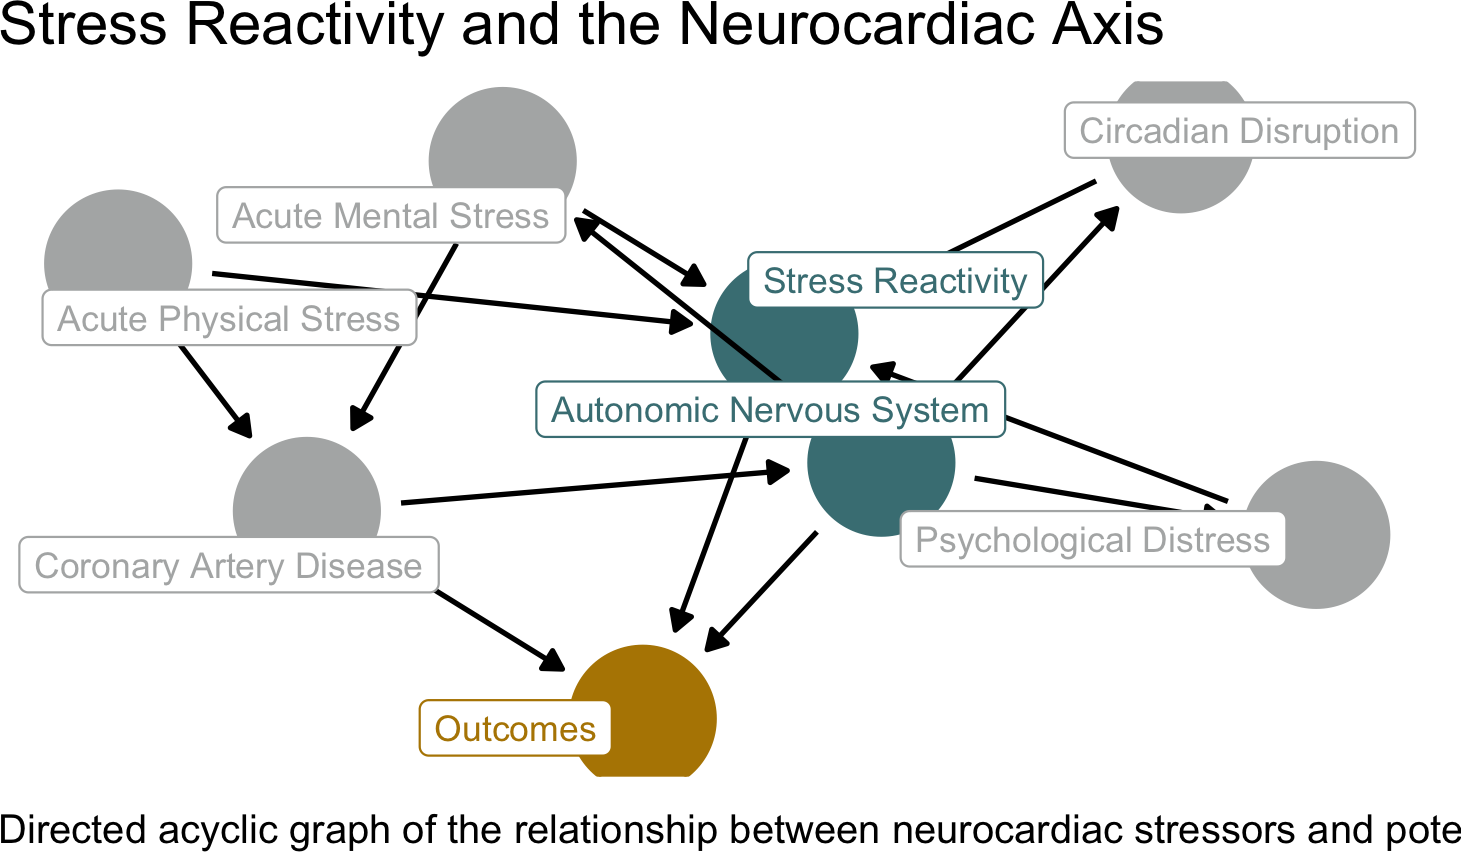
\includegraphics{dissertation_files/figure-latex/unnamed-chunk-13-1.png}

\newpage

\hypertarget{FigurePoincare}{%
\subsection{Poincaré Plot of HRV}\label{FigurePoincare}}

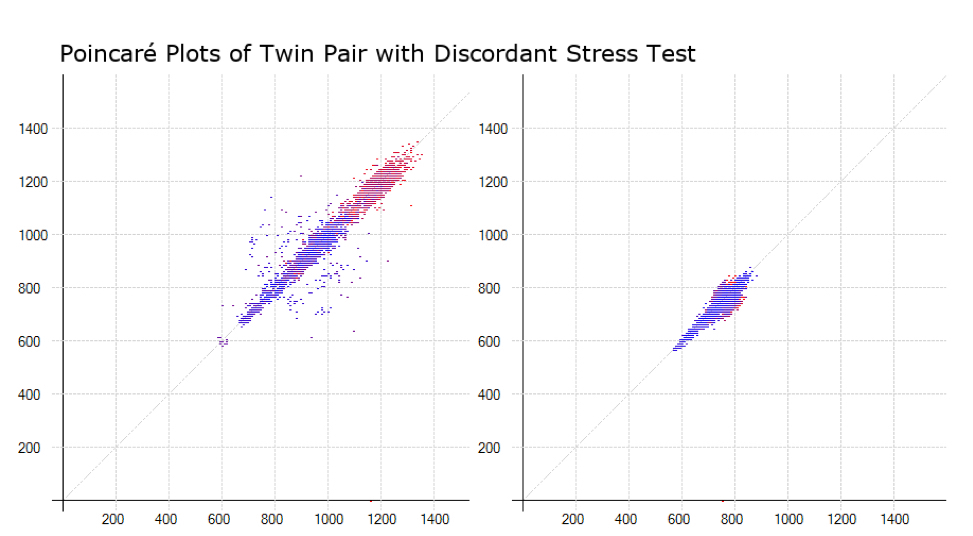
\includegraphics[width=3.24in]{refs/poincare}

\newpage
\bfoot

\hypertarget{TableOneBiobank}{%
\subsection{Biobank Cohort Description}\label{TableOneBiobank}}

\captionsetup[table]{labelformat=empty,skip=1pt}
\begin{longtable}{lc}
\caption*{
\large Emory Cardiovascular Biobank\\ 
\small Cohort Description\\ 
} \\ 
\toprule
\textbf{Characteristic} & \textbf{N = 56}\textsuperscript{1} \\ 
\midrule
Age (years) & 62 (52, 70) \\ 
Race &  \\ 
African American Black & 14 (26\%) \\ 
Asian & 2 (3.8\%) \\ 
Caucasian White & 37 (70\%) \\ 
BMI (kg/m\textasciicircum 2) & 29.3 (26.2, 34.0) \\ 
Sex &  \\ 
Female & 9 (17\%) \\ 
Male & 44 (83\%) \\ 
PHQ-9 Score & 4.5 (1.0, 9.0) \\ 
Depression & 10 (21\%) \\ 
Gensini Score & 26 (20, 51) \\ 
Stenosis & 34 (71\%) \\ 
CASS-70 Score &  \\ 
0 & 21 (44\%) \\ 
1 & 13 (27\%) \\ 
2 & 9 (19\%) \\ 
3 & 5 (10\%) \\ 
\bottomrule
\end{longtable}
\vspace{-5mm}
\begin{minipage}{\linewidth}
\textsuperscript{1}Median (IQR); n (\%) \\ 
\end{minipage}
\begin{minipage}{\linewidth}
A description of subjects undergoing left heart catheterization with coronary angiography, including burden of coronary artery disease. CASS = Coronary Artery Surgery Score, PHQ = Patient Health Questionnaire, BMI = Body Mass Index.\\ 
\end{minipage}

\efoot
\newpage
\bland
\bfoot

\hypertarget{TableOneTwins}{%
\subsection{Twin Cohorts Description}\label{TableOneTwins}}

\captionsetup[table]{labelformat=empty,skip=1pt}
\begin{longtable}{lcccc}
\caption*{
\large Emory Twins Study\\ 
\small Cohort Discription\\ 
} \\ 
\toprule
\textbf{Characteristic} & \textbf{THS1}, N = 361\textsuperscript{1} & \textbf{SAVEIT}, N = 206\textsuperscript{1} & \textbf{THS2}, N = 165\textsuperscript{1} & \textbf{ETSF}, N = 280\textsuperscript{1} \\ 
\midrule
Age (years) & 55.0 (52.0, 57.0) & 57.0 (56.0, 59.0) & 61.0 (59.0, 62.0) & 68.4 (66.8, 69.5) \\ 
BMI (kg/m\textasciicircum 2) & 28.0 (26.0, 32.0) & 30.0 (27.0, 33.0) & 30.0 (27.0, 33.0) & 29.0 (27.0, 32.0) \\ 
Race &  &  &  &  \\ 
White & 345 (96\%) & 198 (96\%) & 157 (95\%) & 269 (96\%) \\ 
African American & 12 (3.3\%) & 8 (3.9\%) & 6 (3.6\%) & 7 (2.5\%) \\ 
Asian & 4 (1.1\%) & 0 (0\%) & 2 (1.2\%) & 4 (1.4\%) \\ 
Current Smoker & 230 (64\%) & 155 (76\%) & 120 (74\%) & 178 (64\%) \\ 
Known IHD & 34 (9.4\%) & 30 (15\%) & 29 (18\%) & 11 (3.9\%) \\ 
Congestive Heart Failure & 2 (0.6\%) & 0 (0\%) & 3 (1.8\%) & 4 (1.4\%) \\ 
Hypertension & 106 (29\%) & 69 (33\%) & 91 (55\%) & 165 (59\%) \\ 
Diabetes Mellitus & 33 (9.1\%) & 34 (17\%) & 27 (16\%) & 64 (23\%) \\ 
Post-Traumatic Stress Disorder & 22 (6.1\%) & 59 (29\%) & 45 (27\%) & 41 (15\%) \\ 
Depression & 40 (11\%) & 42 (20\%) & 26 (16\%) & 27 (9.7\%) \\ 
Abnormal Myocardial Perfusion & 40 (13\%) & 10 (5.9\%) & 29 (18\%) & 32 (12\%) \\ 
\bottomrule
\end{longtable}
\vspace{-5mm}
\begin{minipage}{\linewidth}
\textsuperscript{1}Median (IQR); n (\%) \\ 
\end{minipage}
\begin{minipage}{\linewidth}
Description of the veteran twin subjects within each follow-up period. They were evaluated for clinical characteristics, including quantitative myocardial perfusion imaging. THS = Twins Heart Study, SAVEIT = Stress and Vascular Evaluation in Twins, ETSF = Emory Twins Study Follow-Up.\\ 
\end{minipage}

\efoot
\eland
\newpage
\bland
\bfoot

\hypertarget{TableOneMIMS}{%
\subsection{Mental Stress Cohorts Description}\label{TableOneMIMS}}

\captionsetup[table]{labelformat=empty,skip=1pt}
\begin{longtable}{lcccc}
\caption*{
\large MIMS and MIPS\\ 
\small Cohort Discription\\ 
} \\ 
\toprule
 & \multicolumn{2}{c}{MIMS} & \multicolumn{2}{c}{MIPS} \\ 
 \cmidrule(lr){2-3} \cmidrule(lr){4-5}
Characteristic & \textbf{MSIMI = 0}, N = 256\textsuperscript{1} & \textbf{MSIMI = 1}, N = 50\textsuperscript{1} & \textbf{MSIMI = 0}, N = 440\textsuperscript{1} & \textbf{MSIMI = 1}, N = 188\textsuperscript{1} \\ 
\midrule
Age (years) & 52.0 (47.0, 56.2) & 51.5 (46.6, 54.7) & 66 (58, 71) & 64 (57, 71) \\ 
Sex (Female) & 117 (46\%) & 33 (66\%) & 92 (21\%) & 76 (40\%) \\ 
Race &  &  &  &  \\ 
White & 79 (31\%) & 9 (18\%) & 308 (70\%) & 115 (61\%) \\ 
Black & 165 (64\%) & 36 (72\%) & 110 (25\%) & 67 (36\%) \\ 
Other & 12 (4.7\%) & 5 (10\%) & 22 (5.0\%) & 6 (3.2\%) \\ 
BMI (kg/m\textasciicircum 2) & 30 (26, 35) & 30 (26, 38) & 29.1 (25.6, 32.1) & 29.5 (26.2, 32.8) \\ 
Current Smoker & 62 (25\%) & 11 (22\%) & 215 (49\%) & 84 (45\%) \\ 
Obstructive Coronary Artery Disease & 201 (84\%) & 41 (89\%) & 316 (83\%) & 132 (85\%) \\ 
Diabetes Mellitus & 79 (31\%) & 18 (36\%) & 137 (31\%) & 69 (37\%) \\ 
Coronary Artery Bypass Graft & 51 (20\%) & 12 (24\%) & 139 (32\%) & 75 (40\%) \\ 
Percutaneous Coronary Intervention & 177 (69\%) & 35 (70\%) & 226 (51\%) & 100 (53\%) \\ 
Hyperlipidemia & 206 (80\%) & 40 (80\%) & 369 (84\%) & 151 (80\%) \\ 
Hypertension & 205 (80\%) & 42 (84\%) & 325 (74\%) & 147 (78\%) \\ 
PSIMI & 49 (20\%) & 20 (40\%) & 121 (28\%) & 96 (53\%) \\ 
Depression & 92 (37\%) & 16 (32\%) & 111 (26\%) & 51 (28\%) \\ 
Post-Traumatic Stress Disorder & 32 (13\%) & 12 (24\%) & 35 (8.2\%) & 8 (4.4\%) \\ 
\bottomrule
\end{longtable}
\vspace{-5mm}
\begin{minipage}{\linewidth}
\textsuperscript{1}Median (IQR); n (\%) \\ 
\end{minipage}
\begin{minipage}{\linewidth}
MSIMI = Mental Stress Induced Myocardial Ischemia; PSIMI = Physical Stress Induced Myocardial Ischemia, MIMS = Myocardial Infarction and Mental Stress, MIPS = Mental Stress Ischemia Mechanisms and Prognosis Study\\ 
\end{minipage}

\efoot
\eland
\newpage
\bland
\bfoot

\hypertarget{TableTwinsHRV}{%
\subsection{HRV in Twins Cohorts}\label{TableTwinsHRV}}

\captionsetup[table]{labelformat=empty,skip=1pt}
\begin{longtable}{lcccc}
\caption*{
\large Description of HRV\\ 
\small Emory Twins Study\\ 
} \\ 
\toprule
\textbf{ECG/HRV Metric} & \textbf{THS1}\textsuperscript{1} & \textbf{SAVEIT}\textsuperscript{1} & \textbf{THS2}\textsuperscript{1} & \textbf{ETSF}\textsuperscript{1} \\ 
\midrule
RR Interval & 918 (816, 1,018) & 870 (774, 973) & 923 (828, 1,025) & 915 (806, 1,020) \\ 
SDNN & 60 (46, 74) & 52 (40, 68) & 53 (40, 68) & 48 (36, 62) \\ 
RMSSD & 27 (20, 35) & 24 (17, 33) & 25 (18, 35) & 25 (18, 37) \\ 
PNN50 & 0.05 (0.02, 0.11) & 0.03 (0.01, 0.09) & 0.04 (0.01, 0.10) & 0.03 (0.01, 0.09) \\ 
Ultra Low Frequency & 6.60 (5.87, 7.21) & 6.39 (5.68, 7.08) & 6.42 (5.73, 7.11) & 6.00 (5.30, 6.67) \\ 
Very Low Frequency & 7.81 (7.27, 8.25) & 7.55 (7.03, 8.08) & 7.54 (7.02, 8.05) & 7.29 (6.76, 7.79) \\ 
Low Frequency & 6.79 (6.28, 7.23) & 6.57 (6.00, 7.08) & 6.45 (5.85, 6.95) & 6.28 (5.70, 6.86) \\ 
High Frequency & 5.48 (4.94, 6.00) & 5.30 (4.64, 5.92) & 5.31 (4.66, 6.03) & 5.32 (4.64, 6.11) \\ 
Low/High Frequency Ratio & 4.13 (2.63, 6.05) & 4.02 (2.50, 5.92) & 3.24 (2.02, 5.16) & 3.01 (1.71, 4.83) \\ 
Total Power & 8.45 (7.94, 8.86) & 8.20 (7.70, 8.70) & 8.18 (7.69, 8.67) & 7.97 (7.47, 8.46) \\ 
Acceleration Capacity & -11.0 (-14.1, -7.9) & -9.5 (-12.5, -6.9) & -9.4 (-12.2, -6.7) & -8.1 (-11.6, -6.1) \\ 
Deceleration Capacity & 10.3 (7.0, 13.5) & 8.8 (6.1, 11.8) & 8.5 (5.9, 11.4) & 7.3 (5.2, 10.8) \\ 
Sample Entropy & 1.52 (1.33, 1.69) & 1.50 (1.32, 1.70) & 1.53 (1.32, 1.72) & 1.55 (1.35, 1.77) \\ 
Approximate Entropy & 0.93 (0.87, 1.00) & 0.95 (0.89, 1.03) & 0.94 (0.87, 1.01) & 0.96 (0.89, 1.04) \\ 
DYX & 2.91 (2.37, 3.47) & 2.80 (2.31, 3.33) & 2.81 (2.30, 3.34) & 2.58 (2.03, 3.13) \\ 
\bottomrule
\end{longtable}
\vspace{-5mm}
\begin{minipage}{\linewidth}
\textsuperscript{1}Median (IQR) \\ 
\end{minipage}
\begin{minipage}{\linewidth}
Heart rate variability is described in each of the follow-up periods. HRV = heart rate variability, Dyx = kurtosis of Poincare plot, SDNN = the standard deviation of normally conducted RR intervals, RMSSD = the root mean square of successive differences in normally conducted RR intervals, PNN50 = proportion of normally conducted RR intervals that differ by more than 50 ms divided by the total number of normally conducted RR intervals\\ 
\end{minipage}

\efoot
\eland
\newpage

\hypertarget{myocardial-ischemia-2}{%
\section{Myocardial Ischemia}\label{myocardial-ischemia-2}}

\emph{The follow section divides the relevant figures and tables into those that pertain to the relationship of autonomic function and myocardial ischemia, including both obstructive coronary artery disease and myocardial perfusion.}

\newpage
\bland
\bfoot

\hypertarget{TableBiobankCAD}{%
\subsection{Relationship Between Obstructive and Non-Obstructive Coronary Artery Disease}\label{TableBiobankCAD}}

\captionsetup[table]{labelformat=empty,skip=1pt}
\begin{longtable}{lccc}
\caption*{
\large HRV and Obstructive CAD\\ 
\small Emory Cardiovascular Biobank\\ 
} \\ 
\toprule
\textbf{Characteristic} & \textbf{Nonobstructive CAD}, N = 29\textsuperscript{1} & \textbf{Obstructive CAD}, N = 27\textsuperscript{1} & \textbf{p-value}\textsuperscript{2} \\ 
\midrule
RR Interval & 733 (655, 932) & 868 (786, 922) & 0.12 \\ 
SDNN & 27 (17, 54) & 43 (26, 52) & 0.3 \\ 
RMSSD & 21 (15, 33) & 29 (19, 43) & 0.3 \\ 
PNN50 & 0.02 (0.01, 0.07) & 0.06 (0.02, 0.10) & 0.2 \\ 
Ultra Low Frequency & 141 (86, 294) & 202 (133, 497) & 0.2 \\ 
Very Low Frequency & 474 (158, 1,687) & 887 (444, 1,347) & 0.3 \\ 
Low Frequency & 184 (56, 923) & 486 (138, 704) & 0.4 \\ 
High Frequency & 193 (94, 865) & 327 (148, 687) & 0.4 \\ 
Low/High Frequency Ratio & 1.08 (0.49, 1.76) & 1.42 (0.73, 1.92) & 0.3 \\ 
Total Power & 1,005 (378, 4,144) & 1,915 (929, 3,914) & 0.4 \\ 
Acceleration Capacity & -4.71 (-9.54, -3.85) & -7.04 (-10.08, -4.25) & 0.4 \\ 
Deceleration Capacity & 4.84 (3.85, 9.36) & 6.20 (3.98, 8.96) & 0.6 \\ 
Sample Entropy & 1.36 (1.07, 1.47) & 1.37 (1.18, 1.61) & 0.3 \\ 
Approximate Entropy & 0.94 (0.87, 1.04) & 0.88 (0.85, 1.03) & 0.3 \\ 
Dyx & 1.72 (1.19, 2.11) & 2.07 (1.60, 2.66) & 0.093 \\ 
\bottomrule
\end{longtable}
\vspace{-5mm}
\begin{minipage}{\linewidth}
\textsuperscript{1}Median (IQR) \\ 
\textsuperscript{2}Wilcoxon rank sum exact test \\ 
\end{minipage}
\begin{minipage}{\linewidth}
In patients undergoing angiography, HRV metrics were described in those with both obstructive (>70\%) and nonobstructive CAD, and evaluated for differences in distribution. HRV = Heart Rate Variability, CAD = Coronary Artery Disease.\\ 
\end{minipage}

\efoot
\eland
\newpage
\bland
\bfoot

\hypertarget{TableBiobankRevasc}{%
\subsection{Effective of Revascularization on Autonomic Function}\label{TableBiobankRevasc}}

\captionsetup[table]{labelformat=empty,skip=1pt}
\begin{longtable}{lccc}
\caption*{
\large HRV and Revascularization\\ 
\small Emory Cardiovascular Biobank\\ 
} \\ 
\toprule
\textbf{HRV Metric} & \textbf{No Revascularization} N = 14\textsuperscript{1} & \textbf{Revascularization} N = 34\textsuperscript{1} & \textbf{p-value}\textsuperscript{2} \\ 
\midrule
RR Interval & 648 (608, 872) & 868 (775, 932) & 0.019 \\ 
SDNN & 18 (15, 49) & 37 (26, 51) & 0.11 \\ 
RMSSD & 16 (13, 32) & 28 (20, 40) & 0.11 \\ 
PNN50 & 0.01 (0.01, 0.02) & 0.05 (0.01, 0.10) & 0.086 \\ 
Ultra Low Frequency & 99 (56, 269) & 200 (130, 477) & 0.11 \\ 
Very Low Frequency & 205 (94, 1,465) & 826 (414, 1,336) & 0.2 \\ 
Low Frequency & 70 (42, 833) & 383 (145, 689) & 0.2 \\ 
High Frequency & 96 (89, 480) & 306 (140, 620) & 0.2 \\ 
Low/High Frequency Ratio & 0.99 (0.41, 1.28) & 1.45 (0.65, 2.00) & 0.2 \\ 
Total Power & 431 (216, 3,156) & 1,865 (881, 3,562) & 0.2 \\ 
Acceleration Capacity & -4.12 (-7.06, -2.08) & -6.52 (-9.39, -4.06) & 0.3 \\ 
Deceleration Capacity & 4.83 (2.05, 6.49) & 5.07 (4.00, 8.58) & 0.4 \\ 
Sample Entropy & 1.14 (1.06, 1.39) & 1.37 (1.16, 1.56) & 0.15 \\ 
Approximate Entropy & 0.95 (0.91, 1.11) & 0.92 (0.85, 1.00) & 0.2 \\ 
Dyx & 1.36 (1.17, 1.78) & 2.03 (1.52, 2.71) & 0.063 \\ 
\bottomrule
\end{longtable}
\vspace{-5mm}
\begin{minipage}{\linewidth}
\textsuperscript{1}Median (IQR) \\ 
\textsuperscript{2}Wilcoxon rank sum exact test \\ 
\end{minipage}
\begin{minipage}{\linewidth}
In patients undergoing angiography, HRV metrics were described in those that received revascularization, and evaluated for differences in distribution. HRV = Heart Rate Variability, CAD = Coronary Artery Disease.\\ 
\end{minipage}

\efoot
\eland
\newpage
\bland
\bfoot

\hypertarget{TableBiobankTiming}{%
\subsection{HRV by Timing of Revascularization}\label{TableBiobankTiming}}

\captionsetup[table]{labelformat=empty,skip=1pt}
\begin{longtable}{lcccccc}
\caption*{
\large HRV and Timing of Myocardial Reperfusion\\ 
\small Emory Cardiovascular Biobank\\ 
} \\ 
\toprule
 & \multicolumn{3}{c}{\textbf{No Revascularization}} & \multicolumn{3}{c}{\textbf{Revascularization}} \\ 
 \cmidrule(lr){2-4} \cmidrule(lr){5-7}
\textbf{ECG Metrics} & \textbf{Angiography} N = 6\textsuperscript{1} & \textbf{Before} N = 5\textsuperscript{1} & \textbf{p-value}\textsuperscript{2} & \textbf{Balloon} N = 15\textsuperscript{1} & \textbf{Before} N = 20\textsuperscript{1} & \textbf{p-value}\textsuperscript{2} \\ 
\midrule
RR Interval & 711.7 (688.2, 855.9) & 749.3 (723.6, 869.5) & 0.8 & 849.5 (746.4, 949.6) & 865.8 (801.1, 925.2) & 0.6 \\ 
SDNN & 38.2 (16.8, 60.9) & 47.4 (19.0, 49.0) & >0.9 & 30.7 (22.4, 62.4) & 32.9 (25.5, 51.3) & 0.8 \\ 
RMSSD & 28.8 (14.4, 48.6) & 30.2 (20.6, 38.7) & >0.9 & 21.1 (16.3, 35.2) & 20.7 (15.7, 27.8) & 0.9 \\ 
PNN50 & 0.0 (0.0, 0.1) & 0.0 (0.0, 0.1) & >0.9 & 0.0 (0.0, 0.1) & 0.0 (0.0, 0.0) & 0.6 \\ 
Ultra Low Frequency & 110.3 (36.3, 177.9) & 96.2 (92.7, 185.2) & 0.8 & 151.6 (78.6, 623.7) & 99.3 (52.1, 368.8) & 0.5 \\ 
Very Low Frequency & 684.7 (115.1, 2,018.6) & 1,000.1 (118.5, 1,340.7) & >0.9 & 507.3 (313.6, 1,643.5) & 490.8 (230.2, 1,425.3) & 0.7 \\ 
Low Frequency & 608.7 (74.9, 1,139.7) & 867.6 (48.6, 875.5) & 0.8 & 241.8 (83.9, 530.6) & 276.2 (77.5, 551.9) & >0.9 \\ 
High Frequency & 539.6 (132.5, 967.8) & 387.0 (127.5, 591.6) & 0.8 & 107.7 (68.8, 579.8) & 150.6 (92.7, 322.5) & >0.9 \\ 
Low/High Frequency Ratio & 0.6 (0.4, 1.1) & 1.8 (0.4, 2.2) & 0.4 & 1.2 (0.4, 1.8) & 1.1 (0.5, 2.9) & 0.6 \\ 
Total Power & 1,941.4 (360.8, 4,653.2) & 2,559.9 (363.5, 3,097.1) & >0.9 & 1,208.3 (600.6, 4,185.2) & 1,109.0 (672.4, 2,980.9) & 0.7 \\ 
Acceleration Capacity & -7.3 (-9.5, -4.6) & -4.8 (-11.5, -4.3) & >0.9 & -5.0 (-7.1, -3.8) & -6.4 (-8.8, -3.7) & 0.6 \\ 
Deceleration Capacity & 7.1 (4.7, 9.5) & 6.4 (4.4, 12.1) & >0.9 & 4.4 (3.6, 6.8) & 5.9 (3.8, 7.5) & 0.7 \\ 
Sample Entropy & 1.0 (0.7, 1.4) & 1.4 (0.8, 1.5) & 0.7 & 1.2 (1.0, 1.4) & 1.3 (1.2, 1.5) & 0.2 \\ 
Approximate Entropy & 0.8 (0.7, 1.1) & 0.8 (0.8, 0.9) & >0.9 & 0.9 (0.8, 1.0) & 0.9 (0.8, 1.0) & 0.9 \\ 
\bottomrule
\end{longtable}
\vspace{-5mm}
\begin{minipage}{\linewidth}
\textsuperscript{1}Median (IQR) \\ 
\textsuperscript{2}Wilcoxon rank sum exact test \\ 
\end{minipage}
\begin{minipage}{\linewidth}
HRV was measured before the procedure started and during the time of coronary angiography (versus intervention). Coronary arteries with obstructive disease are reperfused using balloon angioplasty and potential stenting. HRV = Heart Rate Variability, CAD = Coronary Artery Disease.\\ 
\end{minipage}

\efoot
\eland
\newpage
\bland
\bfoot

\hypertarget{TableMimsStress}{%
\subsection{Relationship of HRV with both Mental and Physical Stress}\label{TableMimsStress}}

\captionsetup[table]{labelformat=empty,skip=1pt}
\begin{longtable}{lrrr}
\caption*{
\large Myocardial Perfusion Imaging with Physical and Mental Stress\\ 
\small MIMS/MIPS Cohorts\\ 
} \\ 
\toprule
ECG/HRV Metric & Combined MSIMI/PSIMI\textsuperscript{1} & MSIMI\textsuperscript{1} & PSIMI\textsuperscript{1} \\ 
\midrule
\multicolumn{1}{l}{Heart Rate} \\ 
\midrule
Rest & $1.03$ ($0.92$, $1.16$), AUC $0.51$ & $1.15$ ($1.01$, $1.32$), AUC $0.54$ & $0.97$ ($0.85$, $1.1$), AUC $0.51$ \\ 
Stress & $1$ ($0.9$, $1.1$), AUC $0.49$ & $1.08$ ($0.96$, $1.21$), AUC $0.54$ & $1.02$ ($0.91$, $1.14$), AUC $0.5$ \\ 
Recovery & $0.98$ ($0.88$, $1.1$), AUC $0.52$ & $1.08$ ($0.96$, $1.23$), AUC $0.52$ & $0.95$ ($0.84$, $1.06$), AUC $0.53$ \\ 
\midrule
\multicolumn{1}{l}{T Wave Area} \\ 
\midrule
Rest & $1$ ($0.99$, $1$), AUC $0.49$ & $1$ ($0.98$, $1$), AUC $0.51$ & $1$ ($0.99$, $1$), AUC $0.5$ \\ 
Stress & $1$ ($0.99$, $1.01$), AUC $0.51$ & $1$ ($0.98$, $1.01$), AUC $0.5$ & $1.01$ ($0.99$, $1.02$), AUC $0.52$ \\ 
Recovery & $1$ ($0.99$, $1.01$), AUC $0.51$ & $0.98$ ($0.97$, $1$), AUC $0.56$ & $1$ ($0.99$, $1.01$), AUC $0.5$ \\ 
\midrule
\multicolumn{1}{l}{High Frequency HRV} \\ 
\midrule
Rest & $0.71$ ($0.45$, $1.13$), AUC $0.55$ & $0.57$ ($0.34$, $0.95$), AUC $0.56$ & $0.71$ ($0.43$, $1.17$), AUC $0.54$ \\ 
Stress & $0.7$ ($0.47$, $1.05$), AUC $0.54$ & $0.48$ ($0.31$, $0.76$), AUC $0.58$ & $0.85$ ($0.55$, $1.31$), AUC $0.52$ \\ 
Recovery & $0.82$ ($0.52$, $1.27$), AUC $0.53$ & $0.62$ ($0.38$, $1.02$), AUC $0.55$ & $0.85$ ($0.53$, $1.39$), AUC $0.52$ \\ 
\midrule
\multicolumn{1}{l}{Low Frequency HRV} \\ 
\midrule
Rest & $0.67$ ($0.41$, $1.1$), AUC $0.55$ & $0.53$ ($0.31$, $0.92$), AUC $0.56$ & $0.64$ ($0.37$, $1.08$), AUC $0.54$ \\ 
Stress & $0.64$ ($0.4$, $1.01$), AUC $0.56$ & $0.45$ ($0.27$, $0.74$), AUC $0.59$ & $0.63$ ($0.38$, $1.03$), AUC $0.54$ \\ 
Recovery & $0.64$ ($0.39$, $1.04$), AUC $0.56$ & $0.43$ ($0.25$, $0.74$), AUC $0.59$ & $0.64$ ($0.38$, $1.08$), AUC $0.55$ \\ 
\bottomrule
\end{longtable}
\vspace{-5mm}
\begin{minipage}{\linewidth}
\textsuperscript{1}Logistic regression model, OR with 95\% CI and concordance statistic. \\ 
\end{minipage}
\begin{minipage}{\linewidth}
HRV was measured during the three stages of mental stress challenge and compared in logistic regression models with the results of myocardial perfusion imaging. HRV = heart rate variability, MSIMI = mental stress-induced myocardial ischemia, PSIMI = physical stress-induced myocardial ischemia, AUC = area under receiver-operator curve. Bolded text signifies a p-value < 0.05.\\ 
\end{minipage}

\efoot
\eland
\newpage
\bland
\bfoot

\hypertarget{TableTwinsMPI}{%
\subsection{Quantitative Myocardial Perfusion and HRV}\label{TableTwinsMPI}}

\captionsetup[table]{labelformat=empty,skip=1pt}
\begin{longtable}{lrrrrr}
\caption*{
\large Myocardial Perfusion Imaging and Morning HRV\\ 
\small Emory Twins Study\\ 
} \\ 
\toprule
 & AC & \emph{Dyx} & HF & LF & VLF \\ 
\midrule
\multicolumn{1}{l}{Coronary Flow Reserve} \\ 
\midrule
Model 1 & $0.96$ ($0.95$, $0.98$) & $1.13$ ($1.05$, $1.22$) & $1.10$ ($1.02$, $1.20$) & $1.23$ ($1.11$, $1.35$) & $1.18$ ($1.06$, $1.31$) \\ 
Model 2 & $0.97$ ($0.95$, $0.99$) & $1.09$ ($1.01$, $1.17$) & $1.10$ ($1.02$, $1.20$) & $1.21$ ($1.10$, $1.34$) & $1.17$ ($1.05$, $1.30$) \\ 
Model 3 & $0.97$ ($0.95$, $0.99$) & $1.04$ ($0.96$, $1.12$) & $1.09$ ($1.01$, $1.18$) & $1.16$ ($1.04$, $1.28$) & $1.11$ ($0.99$, $1.24$) \\ 
\midrule
\multicolumn{1}{l}{Abnormal MPI} \\ 
\midrule
Model 1 & $0.96$ ($0.89$, $1.03$) & $0.72$ ($0.53$, $0.99$) & $1.20$ ($0.87$, $1.64$) & $0.93$ ($0.63$, $1.37$) & $0.78$ ($0.51$, $1.20$) \\ 
Model 2 & $0.96$ ($0.90$, $1.04$) & $0.71$ ($0.51$, $0.97$) & $1.19$ ($0.87$, $1.65$) & $0.90$ ($0.61$, $1.34$) & $0.76$ ($0.49$, $1.19$) \\ 
Model 3 & $0.95$ ($0.88$, $1.03$) & $0.70$ ($0.51$, $0.98$) & $1.21$ ($0.87$, $1.66$) & $0.94$ ($0.61$, $1.43$) & $0.79$ ($0.50$, $1.26$) \\ 
\bottomrule
\end{longtable}
\vspace{-5mm}
\begin{minipage}{\linewidth}
\textsuperscript{1}Model 1 = HRV \\ 
\textsuperscript{2}Model 2 = Model 1 + Age + BMI + Race \\ 
\textsuperscript{3}Model 3 = Model 2 + Smoking + HTN + Cardiovascular Disease \\ 
\end{minipage}
\begin{minipage}{\linewidth}
Relationship between abnormal MPI and CFR with HRV. HRV = heart rate variability, MPI = myocardial perfusion imaging, CFR = coronary flow reserve, LF = low frequency HRV, HF = high frequency HRV, VLF = very low frequency HRV, AC = acceleration capacity\\ 
\end{minipage}

\efoot
\eland
\newpage
\bland
\bfoot

\hypertarget{TableTwinsCircMPI}{%
\subsection{Circadian HRV and Myocardial Perfusion}\label{TableTwinsCircMPI}}

\captionsetup[table]{labelformat=empty,skip=1pt}
\begin{longtable}{lrrr}
\caption*{
\large Circadian HRV and Myocardial Perfusion Abnormalities\\ 
\small Emory Twins Study\\ 
} \\ 
\toprule
 & MESOR & Amplitude & Phi \\ 
\midrule
\multicolumn{1}{l}{Coronary Flow Reserve} \\ 
\midrule
High Frequency HRV & $1.1$ ($1.01$, $1.2$) & $1.1$ ($0.98$, $1.23$) & $0.98$ ($0.94$, $1.03$) \\ 
Low Frequency HRV & $1.21$ ($1.09$, $1.34$) & $1.13$ ($0.96$, $1.34$) & $1.02$ ($0.97$, $1.06$) \\ 
Very Low Frequency HRV & $1.12$ ($1.02$, $1.24$) & $1.13$ ($1.01$, $1.26$) & $1.02$ ($0.96$, $1.09$) \\ 
Acceleration Capacity & $0.97$ ($0.95$, $0.99$) & $1.01$ ($0.98$, $1.04$) & $1.03$ ($0.97$, $1.08$) \\ 
RR Intervals & $1$ ($1$, $1$) & $1$ ($1$, $1$) & $1$ ($0.97$, $1.04$) \\ 
Dyx & $1.19$ ($1.08$, $1.31$) & $1.14$ ($0.99$, $1.3$) & $0.98$ ($0.92$, $1.04$) \\ 
\midrule
\multicolumn{1}{l}{Abnormal MPI} \\ 
\midrule
High Frequency HRV & $1.32$ ($0.9$, $1.92$) & $1.88$ ($0.93$, $3.8$) & $0.99$ ($0.81$, $1.2$) \\ 
Low Frequency HRV & $0.88$ ($0.58$, $1.32$) & $1.14$ ($0.61$, $2.15$) & $0.92$ ($0.76$, $1.1$) \\ 
Very Low Frequency HRV & $0.88$ ($0.57$, $1.36$) & $1$ ($0.63$, $1.6$) & $0.96$ ($0.75$, $1.24$) \\ 
Acceleration Capacity & $0.98$ ($0.91$, $1.05$) & $1.14$ ($1.01$, $1.28$) & $0.89$ ($0.7$, $1.15$) \\ 
RR Intervals & $1$ ($1$, $1$) & $1$ ($1$, $1.01$) & $0.92$ ($0.81$, $1.05$) \\ 
Dyx & $0.89$ ($0.61$, $1.31$) & $0.78$ ($0.4$, $1.5$) & $0.88$ ($0.7$, $1.09$) \\ 
\bottomrule
\end{longtable}
\begin{minipage}{\linewidth}
Myocardial perfusion was quantified as a ccontinuous variable and as a binary of abnormal or normal. The HRV metrics are measured over 24 hours using cosinor statistics. MPI = myocardial perfusion imaging, CFR = coronary flow reserve, HRV = heart rate variability, LF = low frequency HRV, HF = high frequency HRV, VLF = very low frequency HRV, AC = acceleration capacity, MESOR = midline estimating statistic of rhythm, Amplitude = maximum distance from MESOR, Phi = shift of acrophase\\ 
\end{minipage}

\efoot
\eland
\newpage

\hypertarget{psychological-stress-2}{%
\section{Psychological Stress}\label{psychological-stress-2}}

\emph{The follow section divides the relevant figures and tables into those that pertain to the relationship of autonomic function and psychological stress, including both acute mental stress and chronic psychological stress.}

\newpage
\bfoot

\hypertarget{depression-by-phq-9-and-hrv}{%
\subsection{Depression by PHQ-9 and HRV}\label{depression-by-phq-9-and-hrv}}

\captionsetup[table]{labelformat=empty,skip=1pt}
\begin{longtable}{lccc}
\caption*{
\large HRV and Depression by PHQ-9\\ 
\small Emory Cardiovascular Biobank\\ 
} \\ 
\toprule
\textbf{HRV Metric} & \textbf{No Depression}, N = 38\textsuperscript{1} & \textbf{Depression}, N = 10\textsuperscript{1} & \textbf{p-value}\textsuperscript{2} \\ 
\midrule
RR Interval & 872 (738, 929) & 727 (689, 920) & 0.6 \\ 
SDNN & 37 (21, 54) & 26 (16, 44) & 0.6 \\ 
RMSSD & 25 (19, 36) & 16 (13, 26) & 0.13 \\ 
PNN50 & 0.03 (0.01, 0.09) & 0.01 (0.01, 0.04) & 0.089 \\ 
Ultra Low Frequency & 233 (108, 405) & 173 (81, 358) & >0.9 \\ 
Very Low Frequency & 887 (310, 1,613) & 444 (227, 1,561) & 0.7 \\ 
Low Frequency & 486 (109, 725) & 138 (67, 617) & 0.6 \\ 
High Frequency & 306 (117, 824) & 99 (51, 316) & 0.14 \\ 
Low/High Frequency Ratio & 1.35 (0.64, 1.90) & 1.28 (1.01, 1.98) & 0.9 \\ 
Total Power & 1,865 (660, 3,914) & 929 (438, 2,786) & 0.5 \\ 
Acceleration Capacity & -6.52 (-10.22, -4.21) & -3.88 (-7.42, -2.64) & 0.3 \\ 
Deceleration Capacity & 5.2 (4.0, 9.0) & 4.0 (3.1, 7.5) & 0.4 \\ 
Sample Entropy & 1.41 (1.14, 1.62) & 1.34 (1.07, 1.50) & 0.4 \\ 
Approximate Entropy & 0.92 (0.85, 1.04) & 0.99 (0.93, 1.04) & 0.4 \\ 
Dyx & 1.75 (1.29, 2.57) & 2.07 (1.76, 2.69) & 0.4 \\ 
\bottomrule
\end{longtable}
\vspace{-5mm}
\begin{minipage}{\linewidth}
\textsuperscript{1}Median (IQR) \\ 
\textsuperscript{2}Wilcoxon rank sum exact test \\ 
\end{minipage}
\begin{minipage}{\linewidth}
In patients undergoing angiography, HRV metrics were described in those with moderate to severe depressive symptoms to those with mild to minimal symptoms by PHQ-9. HRV = Heart Rate Variability, PHQ-9 = Patient Health Questionnaire.\\ 
\end{minipage}

\efoot
\newpage
\bland
\bfoot

\hypertarget{TableTwinsPsych}{%
\subsection{HRV and Chronic Mental Stress in Twins}\label{TableTwinsPsych}}

\captionsetup[table]{labelformat=empty,skip=1pt}
\begin{longtable}{lrrrrr}
\caption*{
\large Morning HRV and Chronic Psychological Stress\\ 
\small Emory Twins Study\\ 
} \\ 
\toprule
 & AC & \emph{Dyx} & HF & LF & VLF \\ 
\midrule
\multicolumn{1}{l}{PTSD} \\ 
\midrule
Model 1 & $1.11$ ($1.03$, $1.21$) & $0.90$ ($0.67$, $1.20$) & $0.69$ ($0.50$, $0.94$) & $0.60$ ($0.42$, $0.86$) & $0.70$ ($0.48$, $1.03$) \\ 
Model 2 & $1.11$ ($1.02$, $1.20$) & $2.12$ ($2.12$, $2.13$) & $0.70$ ($0.51$, $0.97$) & $0.63$ ($0.44$, $0.92$) & $0.75$ ($0.75$, $0.75$) \\ 
Model 3 & $1.15$ ($1.06$, $1.26$) & $1.98$ ($0.44$, $8.89$) & $0.57$ ($0.40$, $0.82$) & $0.65$ ($0.45$, $0.94$) & $0.61$ ($0.40$, $0.94$) \\ 
\midrule
\multicolumn{1}{l}{Depression} \\ 
\midrule
Model 1 & $1.25$ ($1.12$, $1.39$) & $0.60$ ($0.25$, $1.47$) & $0.53$ ($0.16$, $1.78$) & $0.46$ ($0.46$, $0.46$) & $0.22$ ($0.12$, $0.42$) \\ 
Model 2 & $1.25$ ($1.11$, $1.39$) & $0.54$ ($0.16$, $1.86$) & $0.52$ ($0.35$, $0.78$) & $0.25$ ($0.15$, $0.40$) & $0.20$ ($0.11$, $0.36$) \\ 
Model 3 & $1.22$ ($0.71$, $2.08$) & $0.32$ ($0.10$, $0.98$) & $0.41$ ($0.04$, $4.61$) & $0.05$ ($0.00$, $1.21$) & $0.04$ ($0.00$, $0.92$) \\ 
\bottomrule
\end{longtable}
\vspace{-5mm}
\begin{minipage}{\linewidth}
\textsuperscript{1}Model 1 = HRV \\ 
\textsuperscript{2}Model 2 = Model 1 + Age + BMI + Race \\ 
\textsuperscript{3}Model 3 = Model 2 + Smoking + HTN + Cardiovascular Disease \\ 
\end{minipage}
\begin{minipage}{\linewidth}
Depression is measured as a binary outcome with Beck Depression Inventory score > 14. PTSD = Post-Traumatic Stress Disorder, HRV = heart rate variability, LF = low frequency HRV, HF = high frequency HRV, VLF = very low frequency HRV, AC = acceleration capacity\\ 
\end{minipage}

\efoot
\eland
\newpage
\bfoot

\hypertarget{TableTwinsCircPsych}{%
\subsection{Circadian HRV and Chronic Mental Stress}\label{TableTwinsCircPsych}}

\captionsetup[table]{labelformat=empty,skip=1pt}
\begin{longtable}{lrrr}
\caption*{
\large Circadian HRV and Chronic Psychological Stress\\ 
\small Emory Twins Study\\ 
} \\ 
\toprule
 & MESOR & Amplitude & Phi \\ 
\midrule
\multicolumn{1}{l}{PTSD} \\ 
\midrule
High Frequency HRV & $0.61$ ($0.42$, $0.88$) & $0.28$ ($0.09$, $0.84$) & $1.16$ ($0.96$, $1.4$) \\ 
Low Frequency HRV & $0.46$ ($0.31$, $0.69$) & $0.31$ ($0.13$, $0.72$) & $1.02$ ($0.86$, $1.21$) \\ 
Very Low Frequency HRV & $0.56$ ($0.36$, $0.87$) & $0.49$ ($0.28$, $0.86$) & $1.1$ ($0.87$, $1.39$) \\ 
Acceleration Capacity & $1.13$ ($1.03$, $1.25$) & $0.75$ ($0.6$, $0.94$) & $0.87$ ($0.71$, $1.08$) \\ 
RR Intervals & $1$ ($1$, $1$) & $1$ ($1$, $1.01$) & $0.99$ ($0.86$, $1.13$) \\ 
Dyx & $0.67$ ($0.47$, $0.95$) & $0.93$ ($0.57$, $1.51$) & $1.16$ ($0.94$, $1.44$) \\ 
\midrule
\multicolumn{1}{l}{Depression} \\ 
\midrule
High Frequency HRV & $0.43$ ($0.27$, $0.69$) & $0.42$ ($0.22$, $0.82$) & $1.09$ ($0.89$, $1.35$) \\ 
Low Frequency HRV & $0.26$ ($0.15$, $0.45$) & $0.31$ ($0.14$, $0.68$) & $1.06$ ($0.86$, $1.31$) \\ 
Very Low Frequency HRV & $0.24$ ($0.13$, $0.45$) & $0.26$ ($0.13$, $0.5$) & $1.12$ ($0.83$, $1.53$) \\ 
Acceleration Capacity & $1.25$ ($1.11$, $1.41$) & $0.79$ ($0.67$, $0.94$) & $0.94$ ($0.73$, $1.21$) \\ 
RR Intervals & $1$ ($1$, $1$) & $1$ ($1$, $1.01$) & $0.9$ ($0.78$, $1.04$) \\ 
Dyx & $0.35$ ($0.23$, $0.55$) & $0.61$ ($0.33$, $1.12$) & $0.95$ ($0.75$, $1.21$) \\ 
\bottomrule
\end{longtable}
\begin{minipage}{\linewidth}
Depression is measured as a binary outcome with Beck Depression Inventory score > 14. The HRV metrics are measured over 24 hours using cosinor statistics.  PTSD = Post-Traumatic Stress Disorder, HRV = heart rate variability, LF = low frequency HRV, HF = high frequency HRV, VLF = very low frequency HRV, AC = acceleration capacity, MESOR = midline estimating statistic of rhythm, Amplitude = maximum distance from MESOR, Phi = shift of acrophase\\ 
\end{minipage}

\efoot
\newpage

\hypertarget{FigureMimsViolin}{%
\subsection{HRV and Mental Stress Challenge}\label{FigureMimsViolin}}

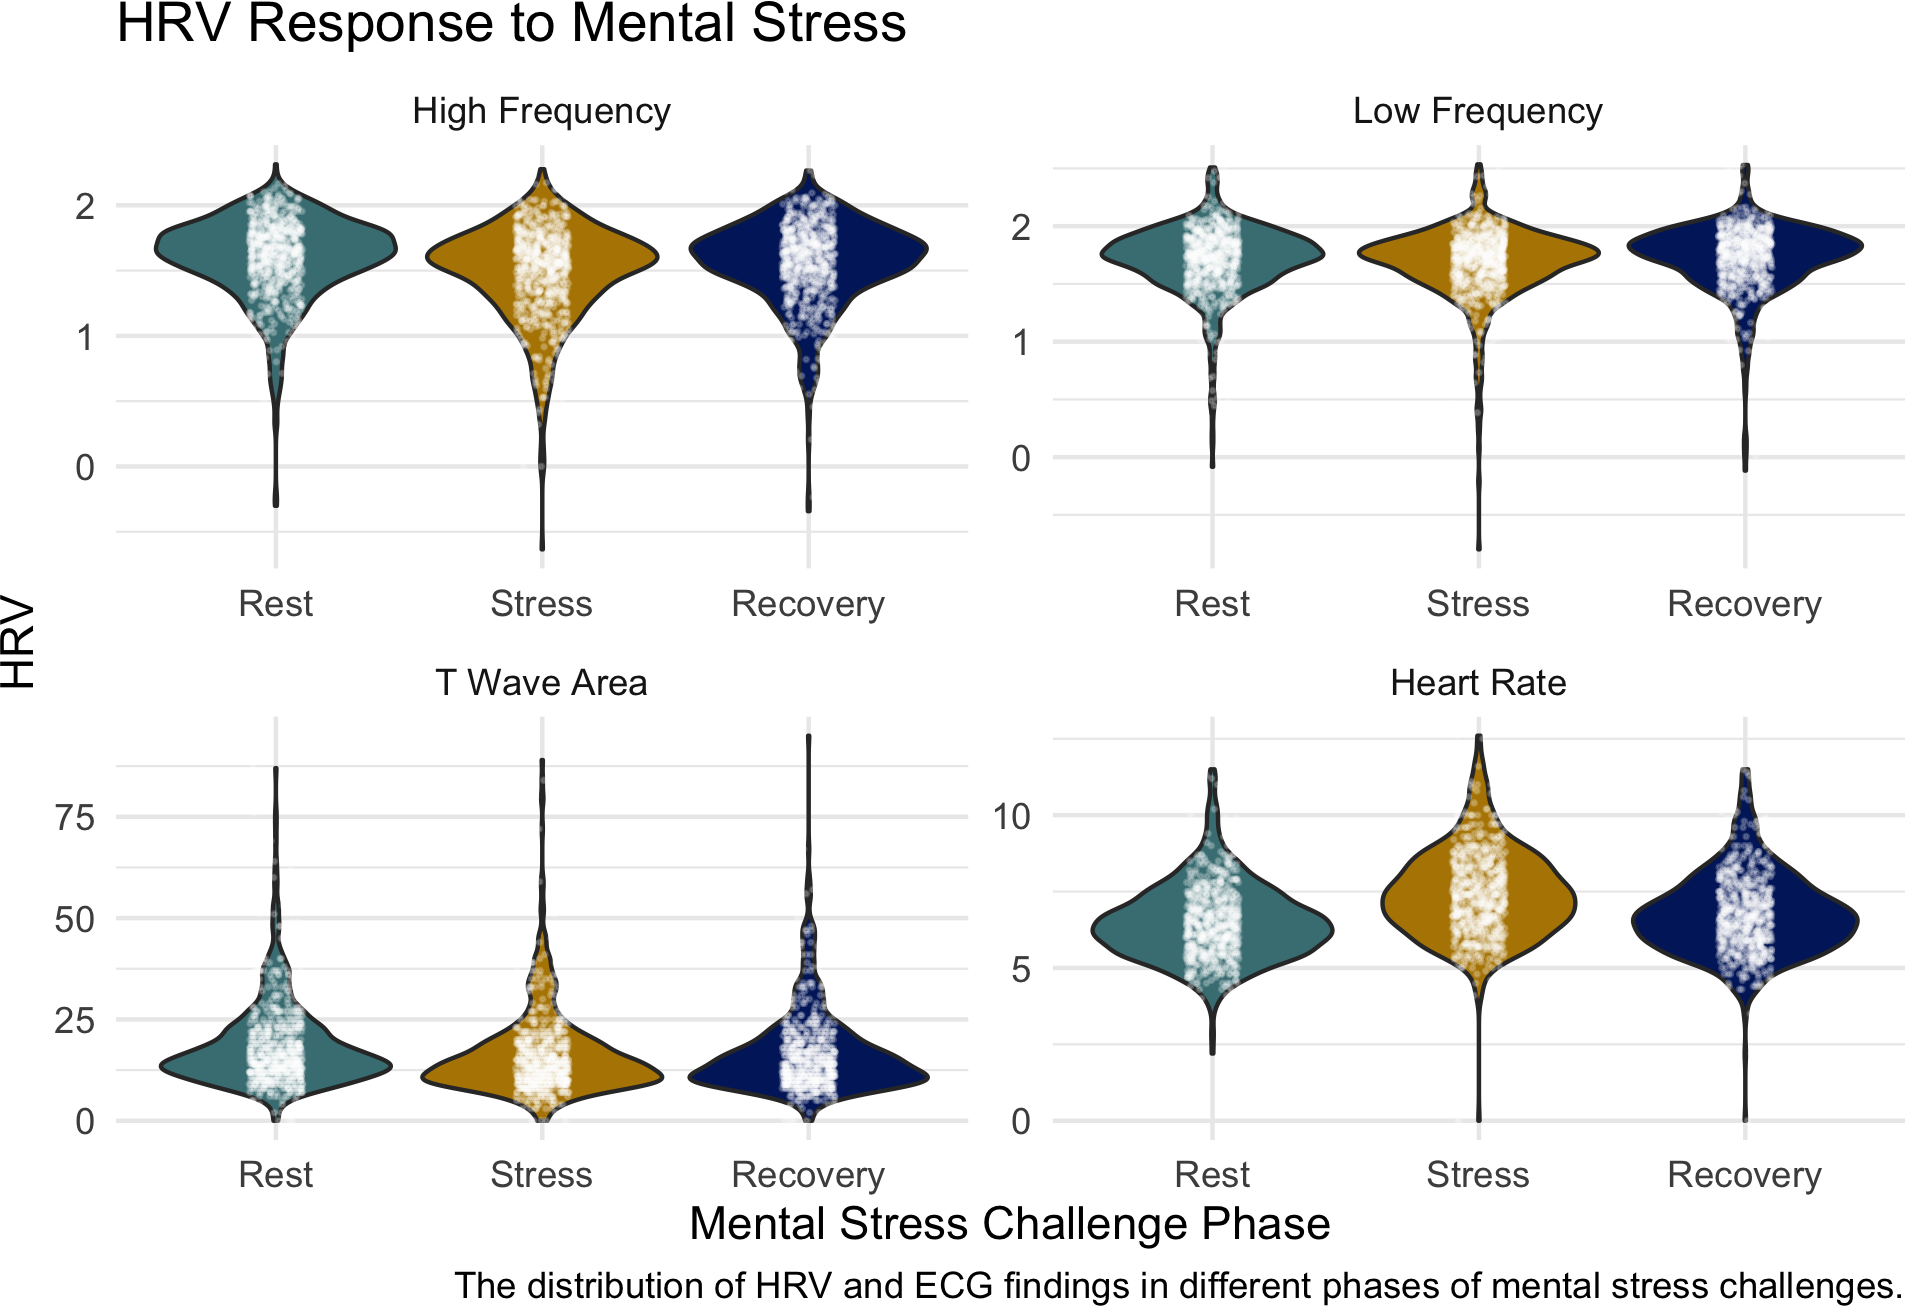
\includegraphics{dissertation_files/figure-latex/unnamed-chunk-28-1.png}

\newpage
\bfoot

\hypertarget{TableMimsPaired}{%
\subsection{Distribution of HRV and Mental Stress Challenge}\label{TableMimsPaired}}

\captionsetup[table]{labelformat=empty,skip=1pt}
\begin{longtable}{lrr}
\caption*{
\large Difference between Mental Stress Challenge Phases and ECG Metrics\\ 
\small MIMS/MIPS Cohorts\\ 
} \\ 
\toprule
 & Mean (95\% CI) & T-statistic \\ 
\midrule
\multicolumn{1}{l}{Heart Rate} \\ 
\midrule
Stress & $1.0$ ($0.9$, $1.0$) & $22.1$ \\ 
Recovery & $0.3$ ($0.2$, $0.3$) & $8.2$ \\ 
\midrule
\multicolumn{1}{l}{High Frequency HRV} \\ 
\midrule
Stress & $-0.1$ ($-0.1$, $-0.1$) & $-11.5$ \\ 
Recovery & $-0.0$ ($-0.1$, $-0.0$) & $-5.7$ \\ 
\midrule
\multicolumn{1}{l}{Low Frequency HRV} \\ 
\midrule
Stress & $-0.0$ ($-0.0$, $-0.0$) & $-3.0$ \\ 
Recovery & $0.0$ ($-0.0$, $0.0$) & $1.9$ \\ 
\midrule
\multicolumn{1}{l}{T Wave Area} \\ 
\midrule
Stress & $-3.7$ ($-5.9$, $-1.5$) & $-3.4$ \\ 
Recovery & $-3.2$ ($-5.2$, $-1.3$) & $-3.3$ \\ 
\bottomrule
\end{longtable}
\begin{minipage}{\linewidth}
HRV summarised during stress and recovery phase of the mental stress challenge were compared to rest HRV. HRV = heart rate variability.\\ 
\end{minipage}

\efoot
\newpage
\bfoot

\hypertarget{TableMimsHRV}{%
\subsection{Distribution of HRV and MSIMI}\label{TableMimsHRV}}

\captionsetup[table]{labelformat=empty,skip=1pt}
\begin{longtable}{lccc}
\caption*{
\large HRV distribution by MSIMI\\ 
\small MIMS/MIPS cohorts\\ 
} \\ 
\toprule
\textbf{Characteristic} & \textbf{MSIMI = 0}, N = 710\textsuperscript{1} & \textbf{MSIMI = 1}, N = 243\textsuperscript{1} & \textbf{p-value}\textsuperscript{2} \\ 
\midrule
\multicolumn{1}{l}{Heart Rate} \\ 
\midrule
Rest & 6.40 (5.60, 7.20) & 6.40 (5.88, 7.50) & 0.090 \\ 
Stress & 7.30 (6.40, 8.30) & 7.50 (6.60, 8.50) & 0.092 \\ 
Recovery & 6.65 (5.90, 7.40) & 6.60 (5.90, 7.80) & 0.5 \\ 
\midrule
\multicolumn{1}{l}{T Wave Area} \\ 
\midrule
Rest & 16 (12, 23) & 16 (12, 23) & 0.8 \\ 
Stress & 14 (10, 19) & 14 (10, 20) & 0.9 \\ 
Recovery & 15 (10, 20) & 13 (9, 19) & 0.024 \\ 
\midrule
\multicolumn{1}{l}{High Frequency HRV} \\ 
\midrule
Rest & 1.65 (1.48, 1.81) & 1.61 (1.39, 1.76) & 0.017 \\ 
Stress & 1.57 (1.34, 1.74) & 1.48 (1.22, 1.65) & <0.001 \\ 
Recovery & 1.62 (1.43, 1.78) & 1.55 (1.35, 1.74) & 0.034 \\ 
\midrule
\multicolumn{1}{l}{Low Frequency HRV} \\ 
\midrule
Rest & 1.76 (1.60, 1.89) & 1.70 (1.49, 1.86) & 0.010 \\ 
Stress & 1.74 (1.59, 1.87) & 1.66 (1.48, 1.81) & <0.001 \\ 
Recovery & 1.79 (1.61, 1.91) & 1.71 (1.52, 1.85) & <0.001 \\ 
\bottomrule
\end{longtable}
\vspace{-5mm}
\begin{minipage}{\linewidth}
\textsuperscript{1}Median (IQR) \\ 
\textsuperscript{2}Wilcoxon rank sum test \\ 
\end{minipage}
\begin{minipage}{\linewidth}
The distribution of HRV between those with MSIMI and those without. The HRV metric are stratified by phase of mental stress challenge. MSIMI = mental stress-induced myocardial ischemia, HRV = heart rate variability.\\ 
\end{minipage}

\efoot
\newpage
\bfoot

\hypertarget{TableMimsPsych}{%
\subsection{Depression and PTSD with Mental Stress Challenge}\label{TableMimsPsych}}

\captionsetup[table]{labelformat=empty,skip=1pt}
\begin{longtable}{lrr}
\caption*{
\large Mental Stress Challenge HRV and Chronic Psychological Stress\\ 
\small MIMS/MIPS Cohorts\\ 
} \\ 
\toprule
ECG/HRV Metric & Depression\textsuperscript{1} & PTSD\textsuperscript{1} \\ 
\midrule
\multicolumn{1}{l}{Heart Rate} \\ 
\midrule
Rest & $1.15$ ($1.01$, $1.3$), AUC $0.55$ & $1.33$ ($1.11$, $1.58$), AUC $0.6$ \\ 
Stress & $1.01$ ($0.9$, $1.13$), AUC $0.51$ & $1.04$ ($0.88$, $1.22$), AUC $0.53$ \\ 
Recovery & $1.09$ ($0.97$, $1.22$), AUC $0.54$ & $1.14$ ($0.96$, $1.35$), AUC $0.56$ \\ 
\midrule
\multicolumn{1}{l}{T Wave Area} \\ 
\midrule
Rest & $1$ ($0.99$, $1.01$), AUC $0.54$ & $1$ ($0.99$, $1.01$), AUC $0.56$ \\ 
Stress & $1.01$ ($1$, $1.02$), AUC $0.5$ & $1.01$ ($1$, $1.03$), AUC $0.5$ \\ 
Recovery & $1.01$ ($1$, $1.02$), AUC $0.54$ & $1.02$ ($1$, $1.03$), AUC $0.58$ \\ 
\midrule
\multicolumn{1}{l}{High Frequency HRV} \\ 
\midrule
Rest & $0.98$ ($0.6$, $1.64$), AUC $0.48$ & $0.6$ ($0.31$, $1.23$), AUC $0.54$ \\ 
Stress & $0.79$ ($0.51$, $1.21$), AUC $0.51$ & $0.63$ ($0.35$, $1.17$), AUC $0.54$ \\ 
Recovery & $0.71$ ($0.44$, $1.15$), AUC $0.52$ & $0.53$ ($0.28$, $1.04$), AUC $0.55$ \\ 
\midrule
\multicolumn{1}{l}{Low Frequency HRV} \\ 
\midrule
Rest & $0.71$ ($0.42$, $1.19$), AUC $0.52$ & $0.58$ ($0.29$, $1.21$), AUC $0.57$ \\ 
Stress & $0.74$ ($0.46$, $1.21$), AUC $0.53$ & $0.63$ ($0.34$, $1.26$), AUC $0.55$ \\ 
Recovery & $0.5$ ($0.29$, $0.83$), AUC $0.54$ & $0.51$ ($0.26$, $1.07$), AUC $0.56$ \\ 
\bottomrule
\end{longtable}
\vspace{-5mm}
\begin{minipage}{\linewidth}
\textsuperscript{1}Logistic regression model, OR with 95\% CI and concordance statistic. \\ 
\end{minipage}
\begin{minipage}{\linewidth}
The association between HRV during mental stress challenge and the chronic psychological stressors of depression and PTSD are described. HRV = heart rate variability.\\ 
\end{minipage}

\efoot
\newpage
\bland
\bfoot

\hypertarget{TableMimsMSIMI}{%
\subsection{Modeling Mental Stress-Induced Myocardial Ischemia and HRV}\label{TableMimsMSIMI}}

\captionsetup[table]{labelformat=empty,skip=1pt}
\begin{longtable}{lrrrr}
\caption*{
\large Mental Stress-Induced Myocardial Ischemia and HRV\\ 
\small MIMS/MIPS Cohorts\\ 
} \\ 
\toprule
Sequential Models & Stress LF & Rest LF & Stress HF & Rest HF \\ 
\midrule
Model 1 & $0.45$ ($0.27$, $0.74$), AUC $0.59$ & $0.53$ ($0.31$, $0.92$), AUC $0.56$ & $0.48$ ($0.31$, $0.76$), AUC $0.58$ & $0.57$ ($0.34$, $0.95$), AUC $0.56$ \\ 
Model 2 & $0.49$ ($0.29$, $0.81$), AUC $0.64$ & $0.59$ ($0.34$, $1.04$), AUC $0.62$ & $0.45$ ($0.28$, $0.72$), AUC $0.64$ & $0.49$ ($0.29$, $0.85$), AUC $0.62$ \\ 
Model 3 & $0.51$ ($0.3$, $0.87$), AUC $0.63$ & $0.64$ ($0.36$, $1.13$), AUC $0.62$ & $0.48$ ($0.29$, $0.77$), AUC $0.64$ & $0.53$ ($0.3$, $0.93$), AUC $0.62$ \\ 
Model 4 & $0.53$ ($0.31$, $0.91$), AUC $0.65$ & $0.65$ ($0.36$, $1.15$), AUC $0.63$ & $0.49$ ($0.3$, $0.79$), AUC $0.65$ & $0.54$ ($0.31$, $0.96$), AUC $0.64$ \\ 
Model 5 & $0.52$ ($0.3$, $0.91$), AUC $0.65$ & $0.66$ ($0.36$, $1.18$), AUC $0.63$ & $0.47$ ($0.29$, $0.77$), AUC $0.66$ & $0.54$ ($0.3$, $0.95$), AUC $0.63$ \\ 
\bottomrule
\end{longtable}
\vspace{-5mm}
\begin{minipage}{\linewidth}
\textsuperscript{1}Model 1 = MSIMI \textasciitilde{} HRV \\ 
\textsuperscript{2}Model 2 = Model 1 + Age + BMI + Sex + Race \\ 
\textsuperscript{3}Model 3 = Model 2 + Smoking + Diabetes + Hypertension + Hyperlipidemia \\ 
\textsuperscript{4}Model 4 = Model 3 + Known Coronary/Peripheral Artery Disease \\ 
\textsuperscript{5}Model 5 = Model 4 + Depression + Post-Traumatic Stress Disorder \\ 
\end{minipage}
\begin{minipage}{\linewidth}
The association between the exposure of HRV with the finding of MSIMI is described. The HRV metric are stratified by phase of mental stress challenge. MSIMI = mental stress-induced myocardial ischemia, HRV = heart rate variability.\\ 
\end{minipage}

\efoot
\eland
\newpage

\hypertarget{clinical-outcomes-2}{%
\section{Clinical Outcomes}\label{clinical-outcomes-2}}

\emph{The follow section divides the relevant figures and tables into those describing the relationship between autonomic dysfunction and clinical outcomes.}

\newpage
\bland
\bfoot

\hypertarget{TableTwinsOutcomes}{%
\subsection{Outcomes in Twins}\label{TableTwinsOutcomes}}

\captionsetup[table]{labelformat=empty,skip=1pt}
\begin{longtable}{lrrrrr}
\caption*{
\large Clinical Outcomes by HRV\\ 
\small Emory Twins Study\\ 
} \\ 
\toprule
 & Acceleration Capacity & Dyx & High Frequency HRV & Low Frequency HRV & Very Low Frequency HRV \\ 
\midrule
\multicolumn{1}{l}{Cardiovascular Death} \\ 
\midrule
Model 1 & $1.04$ ($0.97$, $1.11$) & $0.64$ ($0.51$, $0.81$) & $0.84$ ($0.62$, $1.13$) & $0.75$ ($0.54$, $1.03$) & $0.64$ ($0.44$, $0.92$) \\ 
Model 2 & $1.03$ ($0.96$, $1.1$) & $0.65$ ($0.5$, $0.84$) & $0.81$ ($0.59$, $1.12$) & $0.83$ ($0.58$, $1.18$) & $0.67$ ($0.45$, $1.01$) \\ 
Model 3 & $1.03$ ($0.96$, $1.1$) & $0.66$ ($0.51$, $0.85$) & $0.82$ ($0.6$, $1.13$) & $0.86$ ($0.59$, $1.25$) & $0.68$ ($0.45$, $1.04$) \\ 
Model 4 & $1.03$ ($0.96$, $1.12$) & $0.69$ ($0.53$, $0.9$) & $0.79$ ($0.58$, $1.09$) & $0.86$ ($0.57$, $1.29$) & $0.76$ ($0.5$, $1.18$) \\ 
Model 5 & $1.03$ ($0.95$, $1.12$) & $0.68$ ($0.52$, $0.89$) & $0.8$ ($0.58$, $1.11$) & $0.86$ ($0.57$, $1.29$) & $0.77$ ($0.49$, $1.21$) \\ 
\midrule
\multicolumn{1}{l}{All Cause Mortality} \\ 
\midrule
Model 1 & $1.12$ ($1.01$, $1.23$) & $0.49$ ($0.35$, $0.68$) & $0.72$ ($0.48$, $1.09$) & $0.5$ ($0.33$, $0.75$) & $0.43$ ($0.27$, $0.68$) \\ 
Model 2 & $1.12$ ($1$, $1.26$) & $0.44$ ($0.3$, $0.65$) & $0.64$ ($0.4$, $1.01$) & $0.49$ ($0.31$, $0.79$) & $0.4$ ($0.23$, $0.69$) \\ 
Model 3 & $1.13$ ($1.01$, $1.27$) & $0.39$ ($0.26$, $0.6$) & $0.64$ ($0.41$, $1$) & $0.51$ ($0.32$, $0.83$) & $0.41$ ($0.23$, $0.73$) \\ 
Model 4 & $1.12$ ($1$, $1.26$) & $0.41$ ($0.27$, $0.64$) & $0.66$ ($0.43$, $1.03$) & $0.54$ ($0.32$, $0.9$) & $0.44$ ($0.25$, $0.8$) \\ 
Model 5 & $1.11$ ($0.98$, $1.24$) & $0.41$ ($0.27$, $0.64$) & $0.71$ ($0.45$, $1.12$) & $0.55$ ($0.32$, $0.95$) & $0.49$ ($0.27$, $0.88$) \\ 
\bottomrule
\end{longtable}
\vspace{-5mm}
\begin{minipage}{\linewidth}
\textsuperscript{1}Model 1 = HRV \\ 
\textsuperscript{2}Model 2 = Model 1 + Myocardial Perfusion Imaging \\ 
\textsuperscript{3}Model 3 = Model 2 + Age + BMI + Race \\ 
\textsuperscript{4}Model 4 = Model 3 + Cardiovascular Disease + Hypertension + Diabetes + Smoking \\ 
\textsuperscript{5}Model 5 = Model 4 + Depression + PTSD \\ 
\end{minipage}
\begin{minipage}{\linewidth}
Every unit increased in HRV had the associated hazard ratio (95\% CI) for both overall and cardiovascular mortality. HRV = heart rate variability.\\ 
\end{minipage}

\efoot
\eland
\newpage
\bfoot

\hypertarget{TableTwinsCircOutcomes}{%
\subsection{Circadian Outcomes in Twins}\label{TableTwinsCircOutcomes}}

\captionsetup[table]{labelformat=empty,skip=1pt}
\begin{longtable}{lrrr}
\caption*{
\large Clinical Outcomes by Circadian HRV\\ 
\small Emory Twins Study\\ 
} \\ 
\toprule
 & MESOR & Amplitude & Phi \\ 
\midrule
\multicolumn{1}{l}{All Cause Mortality} \\ 
\midrule
High Frequency HRV & $0.64$ ($0.32$, $1.26$) & $0.73$ ($0.29$, $1.82$) & $1.38$ ($0.95$, $1.99$) \\ 
Low Frequency HRV & $0.32$ ($0.16$, $0.67$) & $0.37$ ($0.12$, $1.15$) & $1.08$ ($0.79$, $1.47$) \\ 
Very Low Frequency HRV & $0.36$ ($0.15$, $0.89$) & $0.31$ ($0.05$, $1.91$) & $1.32$ ($0.81$, $2.16$) \\ 
Acceleration Capacity & $1.15$ ($0.98$, $1.36$) & $0.83$ ($0.61$, $1.13$) & $1.05$ ($0.74$, $1.5$) \\ 
RR Intervals & $1$ ($1$, $1$) & $0.99$ ($0.98$, $1$) & $1.04$ ($0.83$, $1.3$) \\ 
Dyx & $0.34$ ($0.21$, $0.56$) & $0.42$ ($0.22$, $0.79$) & $0.93$ ($0.67$, $1.28$) \\ 
\midrule
\multicolumn{1}{l}{Cardiovascular Death} \\ 
\midrule
High Frequency HRV & $0.83$ ($0.53$, $1.32$) & $0.7$ ($0.17$, $2.85$) & $1.13$ ($0.91$, $1.42$) \\ 
Low Frequency HRV & $0.6$ ($0.33$, $1.07$) & $0.66$ ($0.26$, $1.65$) & $0.96$ ($0.76$, $1.21$) \\ 
Very Low Frequency HRV & $0.64$ ($0.32$, $1.3$) & $0.31$ ($0.04$, $2.27$) & $1.05$ ($0.77$, $1.42$) \\ 
Acceleration Capacity & $1.1$ ($0.97$, $1.25$) & $0.8$ ($0.59$, $1.1$) & $1.11$ ($0.88$, $1.39$) \\ 
RR Intervals & $1$ ($1$, $1$) & $0.99$ ($0.98$, $1$) & $0.97$ ($0.83$, $1.14$) \\ 
Dyx & $0.42$ ($0.28$, $0.62$) & $0.54$ ($0.34$, $0.85$) & $0.88$ ($0.68$, $1.13$) \\ 
\bottomrule
\end{longtable}
\begin{minipage}{\linewidth}
The HRV metrics are measured over 24 hours using cosinor statistics. Every unit increase in HRV had an associated hazard ratio (95\% CI) for both overall and cardiovascular mortality. HRV = heart rate variability, LF = low frequency HRV, HF = high frequency HRV, VLF = very low frequency HRV, AC = acceleration capacity, MESOR = midline estimating statistic of rhythm, Amplitude = maximum distance from MESOR, Phi = shift of acrophase\\ 
\end{minipage}

\efoot
\newpage
\bland
\bfoot

\hypertarget{TableMimsOutcomes}{%
\subsection{Outcomes in MIMS/MIPS}\label{TableMimsOutcomes}}

\captionsetup[table]{labelformat=empty,skip=1pt}
\begin{longtable}{lrrrrrr}
\caption*{
\large Outcomes Analysis for Mental Stress and HRV\\ 
\small Traditional and Recurrent Event Models in MIMS/MIPS\\ 
} \\ 
\toprule
 & Death & Cardiovascular Death & Marginal & PWP Total Time & PWP Gap Time & Anderson Gill \\ 
\midrule
\multicolumn{1}{l}{Stress Low Frequency HRV} \\ 
\midrule
Model 1 & $0.39$ ($0.24$, $0.64$) & $0.32$ ($0.18$, $0.57$) & $0.52$ ($0.34$, $0.8$) & $0.49$ ($0.29$, $0.8$) & $0.51$ ($0.31$, $0.81$) & $0.52$ ($0.34$, $0.8$) \\ 
Model 2 & $0.42$ ($0.25$, $0.68$) & $0.32$ ($0.18$, $0.58$) & $0.54$ ($0.35$, $0.84$) & $0.5$ ($0.3$, $0.85$) & $0.53$ ($0.32$, $0.85$) & $0.54$ ($0.35$, $0.84$) \\ 
Model 3 & $0.37$ ($0.22$, $0.63$) & $0.24$ ($0.12$, $0.46$) & $0.52$ ($0.33$, $0.82$) & $0.47$ ($0.27$, $0.84$) & $0.5$ ($0.3$, $0.84$) & $0.52$ ($0.33$, $0.82$) \\ 
Model 4 & $0.38$ ($0.21$, $0.7$) & $0.25$ ($0.12$, $0.52$) & $0.58$ ($0.36$, $0.95$) & $0.48$ ($0.27$, $0.86$) & $0.51$ ($0.3$, $0.85$) & $0.58$ ($0.36$, $0.95$) \\ 
Model 5 & $0.37$ ($0.2$, $0.7$) & $0.24$ ($0.11$, $0.51$) & $0.51$ ($0.31$, $0.84$) & $0.52$ ($0.28$, $0.94$) & $0.53$ ($0.31$, $0.92$) & $0.51$ ($0.31$, $0.84$) \\ 
Model 6 & $0.4$ ($0.2$, $0.77$) & $0.25$ ($0.11$, $0.56$) & $0.5$ ($0.3$, $0.85$) & $0.54$ ($0.29$, $1$) & $0.55$ ($0.31$, $0.97$) & $0.5$ ($0.3$, $0.85$) \\ 
\midrule
\multicolumn{1}{l}{Stress High Frequency HRV} \\ 
\midrule
Model 1 & $0.45$ ($0.26$, $0.77$) & $0.32$ ($0.17$, $0.61$) & $0.65$ ($0.43$, $0.98$) & $0.51$ ($0.32$, $0.8$) & $0.57$ ($0.38$, $0.85$) & $0.65$ ($0.43$, $0.98$) \\ 
Model 2 & $0.48$ ($0.27$, $0.83$) & $0.32$ ($0.16$, $0.62$) & $0.68$ ($0.44$, $1.04$) & $0.53$ ($0.33$, $0.85$) & $0.6$ ($0.4$, $0.9$) & $0.68$ ($0.44$, $1.04$) \\ 
Model 3 & $0.44$ ($0.25$, $0.78$) & $0.28$ ($0.14$, $0.56$) & $0.64$ ($0.42$, $0.99$) & $0.54$ ($0.33$, $0.87$) & $0.59$ ($0.39$, $0.91$) & $0.64$ ($0.42$, $0.99$) \\ 
Model 4 & $0.5$ ($0.27$, $0.92$) & $0.3$ ($0.14$, $0.65$) & $0.71$ ($0.45$, $1.14$) & $0.55$ ($0.34$, $0.89$) & $0.61$ ($0.4$, $0.94$) & $0.71$ ($0.45$, $1.14$) \\ 
Model 5 & $0.5$ ($0.26$, $0.93$) & $0.3$ ($0.13$, $0.66$) & $0.65$ ($0.4$, $1.07$) & $0.57$ ($0.35$, $0.95$) & $0.63$ ($0.41$, $0.98$) & $0.65$ ($0.4$, $1.07$) \\ 
Model 6 & $0.57$ ($0.3$, $1.12$) & $0.31$ ($0.14$, $0.72$) & $0.66$ ($0.39$, $1.1$) & $0.61$ ($0.37$, $1.03$) & $0.67$ ($0.43$, $1.05$) & $0.66$ ($0.39$, $1.1$) \\ 
\bottomrule
\end{longtable}
\vspace{-5mm}
\begin{minipage}{\linewidth}
\textsuperscript{1}Model 1 = MSIMI \textasciitilde{} HRV \\ 
\textsuperscript{2}Model 2 = Model 1 + MSIMI \\ 
\textsuperscript{3}Model 3 = Model 2 + Age + BMI + Sex + Race \\ 
\textsuperscript{4}Model 4 = Model 3 + Smoking + Diabetes + Hypertension + Hyperlipidemia \\ 
\textsuperscript{5}Model 5 = Model 4 + Known Coronary/Peripheral Artery Disease \\ 
\textsuperscript{6}Model 6 = Model 5 + Depression + Post-Traumatic Stress Disorder \\ 
\end{minipage}
\begin{minipage}{\linewidth}
This summarises the Cox proportional hazard models for both censoring events and for recurrent event analyses. Estimates = HR (95\% CI). Bolded terms signify p-value < 0.05. PWP = Prentice, Williams, and Peterson models, MSIMI = Mental Stress-Induced Myocardial Ischemia, LF = Low Frequency, HF = High Frequency, HRV = Heart Rate Variability\\ 
\end{minipage}

\efoot
\eland
\egroup

\end{document}
